\begin{english}

\chapter{Information Visualization}
\label{cha:infovis}

%%%%%%%%%%%%%%%%%%
%%%%%%%%%%%%%%%%%%

  % Stanford Courses!
  % https://graphics.stanford.edu/wikis/cs448b-11-fall
  
  % By: Stanley Smith Stevens http://en.wikipedia.org/wiki/Level_of_measurement

%%%%%%%%%%%%%%%%%%

In order to create visualizations, fundamental knowledge (theory) about Information Visualization is necessary. This chapter introduces a number of concepts related to the field of Information Visualization in general. It also highlights their importance with respect to the visualization creation process, which forms the main subject of this thesis.


\section{The Visualization Process}
%%%-----------------------------------------------------------------------------

The ultimate purpose of Information Visualization is the acquisition of a mental model of a dataset under investigation. The whole process to reach this goal can be referred to as \emph{The Visualization Process} \cite{WuenscheLobb01}.

\begin{figure}
\centering
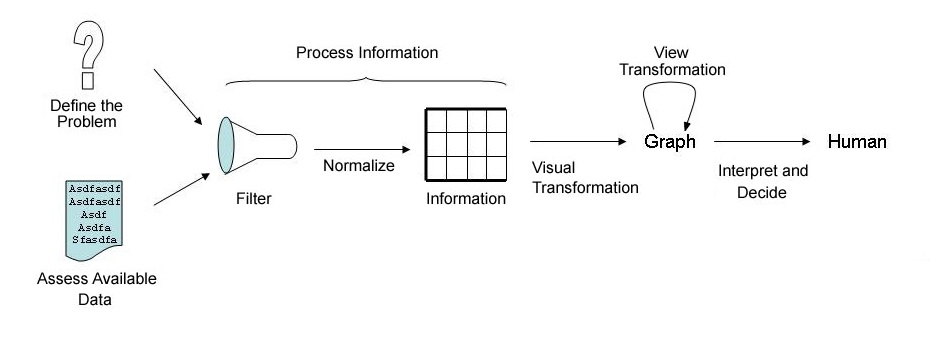
\includegraphics[width=1\textwidth]{visualization_process}
\caption{The Visualization Process}
\label{fig:visprocess}
\end{figure}

This process, as shown in Figure~\ref{fig:visprocess}, involves the creation phase as well as the interpretation of the resulting image by humans in order to gain a mental model and make sense of the data shown. The viewing of a graphical encoding of data should cause an ``Ah-ha!'' reaction in the viewer in the sense that a useful discovery has been made. Information designers can only control the visualization stage with the goal that interpretation of the result is as easy as possible~\cite{Holmberg06}. More specifically, the creation of visualizations involves the application of methods to map data to suitable structures, which can then be encoded through visual properties (like height, size, color etc.).

% We'll examine the respective applicability of interaction for the technologies we investigate.

\section{Computational Support}
%%%-----------------------------------------------------------------------------

According to Spence~\cite{InformationVisualization07}, computers have been responsible for massive advances in the field of Information Visualization.

There are three principal reasons why computational support has huge importance. First, because of \emph{inexpensive and fast memory access}, the storage of truly \emph{vast amounts of data} has become affordable for businesses and governments. Second, with powerful and fast computation mechanisms, the processing of data in realtime enables a number of tasks that are helpful for visually investigating data. Data can be \emph{filtered}, \emph{aggregated} and \emph{transformed} interactively for flexible exploration. This interactivity forms a great advantage of computer-aided visualizations when compared to their equivalents in print, which are static. Users may start exploring information by looking at the whole dataset through an aggregated synoptic view and request details on demand. Third, Spence states that the availability of high resolution graphic displays ensures that the presentation of data matches the power of human visual and cognitive systems. 

Computer graphics is not a new subject, neither is Interactive Information Visualization. Many software products have been developed and released in the last 20-30 years. Among these are graphically intensive \emph{Computer Games}, and \emph{Visual Analysis Tools} targeting all imaginable domains of life. However, in this thesis only technologies that are natively supported by current web browsers are examined, while taking into account the special characteristics of this environment when utilized as a medium. Visualization designers are dealing with a client-server scenario that offers a number of capabilities but also introduces limitations that must be considered.

While the choice of a graphical representation can impact the effectiveness of a visualization, this thesis first and foremost addresses the choice of technology as well as the utilization of suitable methods in terms of software design. A major requirement for all technology options is the support of arbitrary visual representations. Thus, this thesis will give a closer look on both \emph{low level graphical systems} and \emph{higher level visualization frameworks}. It will rather neglect ready-to-use charting libraries which are useful for quickly plotting common data structures but typically lack options for extensive customization. Another key aspect of web-based visualization is the support of interaction, since users can interact with their web-browser using mouse, keyboard or touch surfaces.


\section{The Human User}
%%%-----------------------------------------------------------------------------

With the availability of immense computational power to transform data and create visual output, designers sometimes lose sight of the user being the main consumer of visualizations. As Spence states, visualization is all about how human beings interact with data and how to graphically encode and present data best~\cite{InformationVisualization07}. It is important that the visualization designer is aware of the needs of a user as well as the characteristics of human behavior. This awareness cannot be emphasized enough. A lot of attempts end up in being beautiful, in terms of visually appealing for the eye, but make it hard for the user to make sense of it. Such visualizations are perfectly fine when created in the context of an artistic target, but fail when they are meant to transport information straight away.


\section{The Value of Information Visualization}
%%%-----------------------------------------------------------------------------

Without doubt, the topic of Information Visualization is fascinating, yet the question of its true value is important too~\cite{InformationVisualization07}. This value becomes obvious in many concrete application scenarios.


\subsection{Visual Analytics}
%%%-----------------------------------------------------------------------------

Visual Analytics developed out the fields of Information Visualization and Scientific Visualization and has a strong focus on analytical reasoning.

According to Ziemkiewicz and Kosara~\cite{Ziemkiewicz10}, it combines classical data analysis techniques with those of Information Visualization. In an analysis scenario with the help of Information Visualization users can explore a large amounts of data using visual tools in order to reveal patterns which are not obvious when looking at the raw data.

The importance of Visual Analytics was also recognized by the U.S. Department of Homeland Security when they chartered the National Visualization and Analytics Center (NVAC) in 2004. The goal was to help avoiding future terrorist attacks in the U.S. and around the globe. A lot of groundwork has been done by the NVAC, not least have they contributed a five year research and development agenda for Visual Analytics. \emph{Illuminating the Path - The Research and Development Agenda for Visual Analytics}~\cite{IlluminatingThePath05} addresses the most important needs in R\&D to gain advanced analytical insight. According to them, Visual Analytics is a multidisciplinary field that includes the following focus areas:

\begin{itemize}
\item Analytical reasoning techniques that enable users to obtain deep insights that directly support assessment, planning, and decision making.
\item Visual representations and interaction techniques that take advantage of the human eye's broad bandwidth pathway into the mind to allow users to \emph{see}, \emph{explore}, and \emph{understand} large amounts of information at once.
\item \emph{Data representations} and \emph{transformations} that convert all types of conflicting and dynamic data in ways that support visualization and analysis.
\item Techniques to support \emph{production}, \emph{presentation}, and \emph{dissemination} of the results of an analysis to communicate information in the appropriate context to a variety of audiences.
\end{itemize}

\SuperPar Even though Information Visualization is not limited to the field of Visual Analytics, it is without doubt a major field of application. Thus, techniques and approaches described in this thesis were not developed without bearing Visual Analytics as a main application scenario in mind.


\subsection{Exploratory Data Analysis}
%%%-----------------------------------------------------------------------------


Fluit et. al describe the task of data exploration as a process of information search, that is \emph{not of immediate relevance}~\cite{Fluit05}. The difference between data exploration and querying is that \emph{no particular questions are to be answered}. Instead, users get an \emph{overview} of the complete information available and start to make sense of it by digging deeper into the data and viewing certain aspects, but without losing the overall context. The goal here is that users become familiar with the dataset and figure out how it is structured and organized. Based on knowledge gained through exploration, users are able to formulate specific questions afterwards. In order to make possible Exploratory Data Analysis, \emph{Filtering}, \emph{Zooming} and \emph{Detail-on-demand} functionality must be supported by the visualization.

\subsection{Collaborative Visualization}
%%%-----------------------------------------------------------------------------

\begin{figure}
\centering
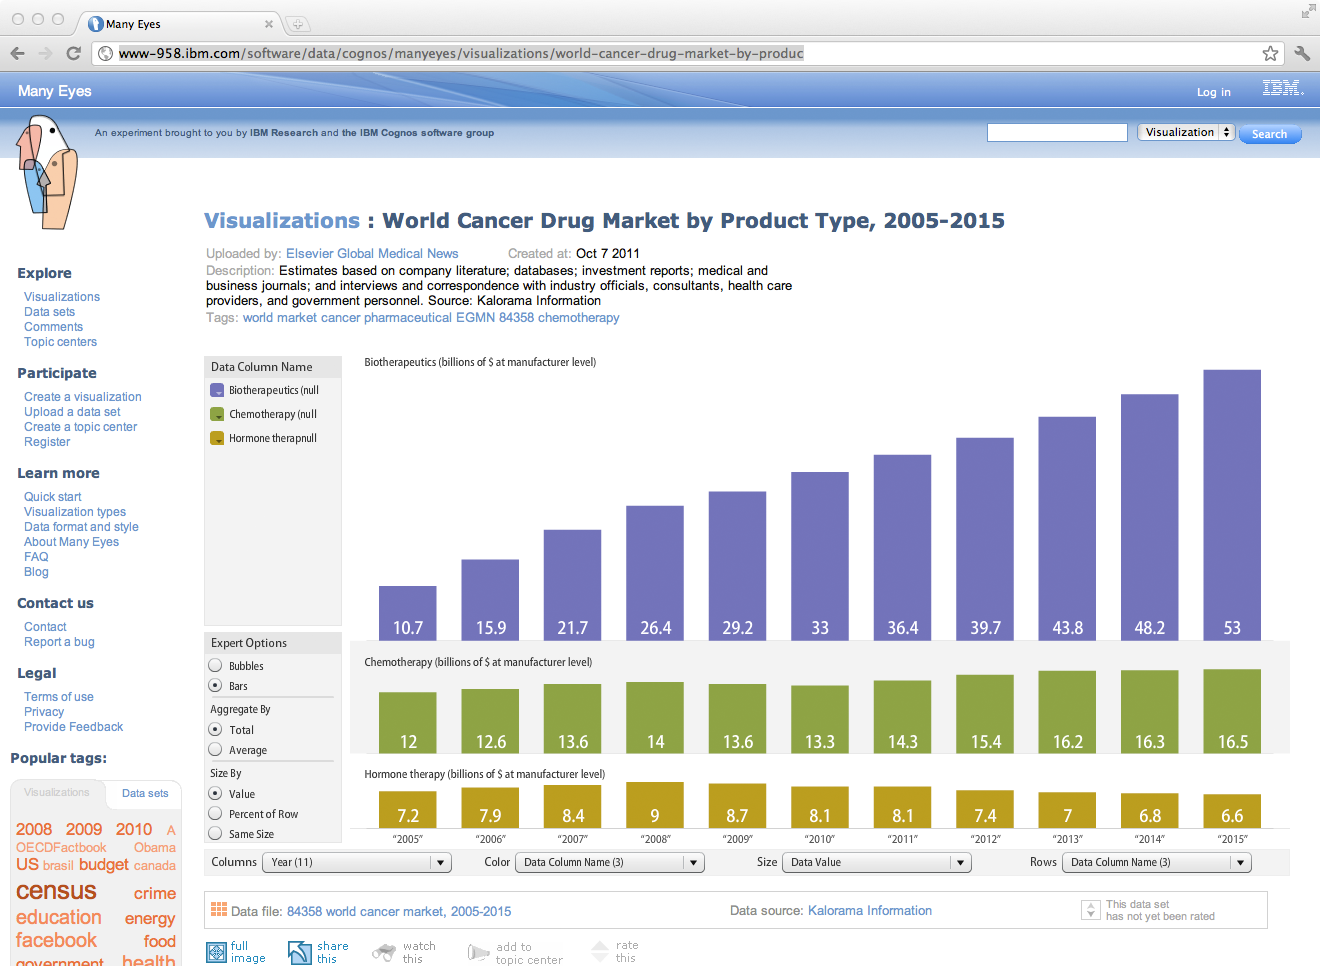
\includegraphics[width=1\textwidth]{manyeyes}
\caption{ManyEyes: Showing a visualization of the World Cancer Drug Market }
\label{fig:manyeyes}
\end{figure}

According to Heer et. al, visualizations are not just analytic tools but social spaces~\cite{voyagers-and-voyeurs,design-considerations-vast}. Visual systems improve our ability to process large amounts of data and enable visual sense-making. Sense-making is a social process, as people interpret data differently~\cite{card99}. This triggers a collective discourse and eventually either leads to consensus or people learn from their peers. Moreover, some datasets are too large to be examined by one person. Using a collaborative interface, a task can be divided into sub-tasks.

Discussions about trends are often scattered and disconnected from the actual visualization~\cite{voyagers-and-voyeurs}. Communication still takes place through email or other classic channels. Resulting from this it is getting difficult for newcomers to catch up and even the review process becomes harder. Thus, discussions should take place right at the visualization workspace.

\begin{figure}
\centering
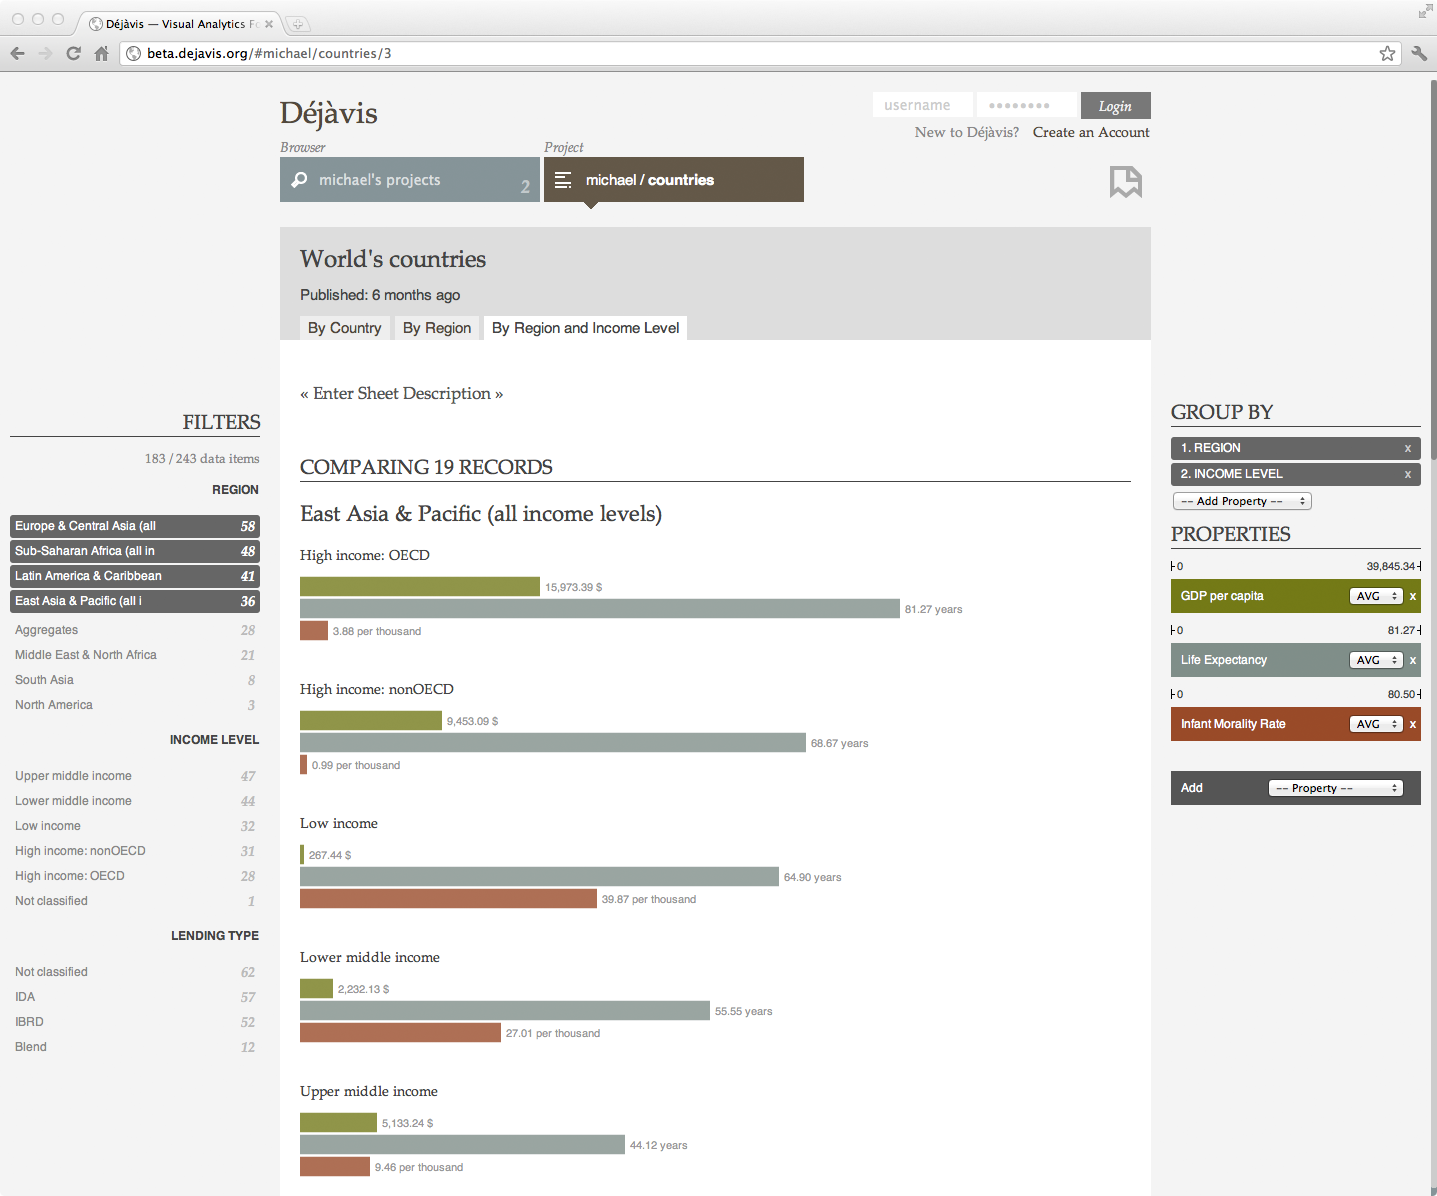
\includegraphics[width=1\textwidth]{dejavis}
\caption{Dejavis: Showing an analysis of the world's countries by various numerical indicators (such as GDP per capita, life expectancy, infant mortality rate).}
\label{fig:dejavis}
\end{figure}

In order to ease the task of exchanging insight discovered on a particular dataset, application bookmarks are important. If the current application state (user settings, data-source) could be stored and made available using a public URL, knowledge can be shared easily with others. This is referred to as \emph{View Sharing} in literature~\cite{clark91}.

A prominent example for such a social data analysis tool is ManyEyes\footnote{http://many-eyes.com}, shown in Figure~\ref{fig:manyeyes}, an IBM research experiment~\cite{manyeyes}. Dejavis\footnote{http://beta.dejavis.org}, as shown in Figure~\ref{fig:dejavis}, is another example, contributed by the author. It supports \emph{View Sharing} \cite{clark91} and \emph{Contextual Data Transformations} \cite{manyeyes}.


\begin{figure}
\centering
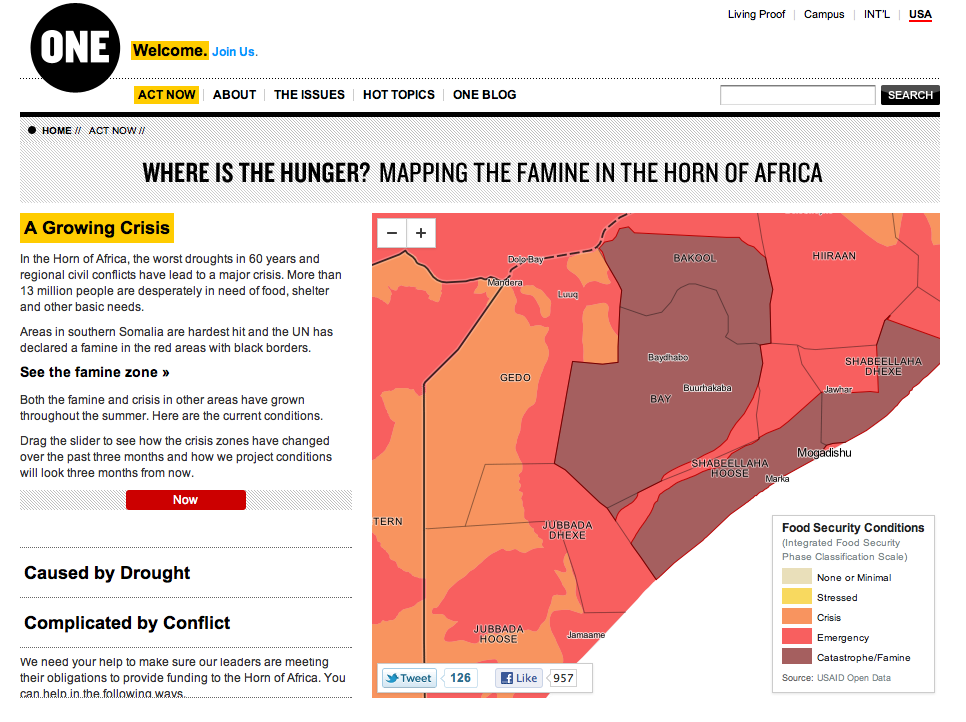
\includegraphics[width=1\textwidth]{horn}
\caption{Where is the Hunger: Mapping the famine in the Horn of Africa.}
\label{fig:horn}
\end{figure}

\subsection{Narrative Visualization}
%%%-----------------------------------------------------------------------------


One promising new field is called Narrative Visualization, which can be described as \emph{telling stories with data}.  Information Visualization, with its ability to reveal narratives within data, is a great way to communicate stories in new different ways~\cite{NarrativeVis10}. Story tellers, like online journalists increasingly start adapting visualizations into their online stories. In some cases the visualization entirely functions in place of a written story. Where is the hunger\footnote{http://one.org/us/actnow/horn.html} (see Figure~\ref{fig:horn}), visually tells the story of the famine in the Horn of Africa.


\section{The Information Seeking Mantra}
%%%-----------------------------------------------------------------------------

According to Shneiderman~\cite{shneiderman96eyes} the bandwidth of information presentation is potentially higher in the visual domain than in any other media. After having completed many projects, he has identified the following principle that applies to the majority of visualization scenarios:

\begin{quotation}
    ``Overview first, zoom and filter, then details-on-demand''
\end{quotation}

\SuperPar This principle is referred to as \emph{The Information Seeking Mantra} and serves as a starting point for creating visualizations. Based on that, Shneiderman also proposes a Task by Data Type Taxonomy (TTT) with seven data types (1-, 2-, 3-dimensional data, temporal data, multi-dimensional data, and tree and network data) and seven tasks (overview, zoom, filter, details-on-demand, relate, history, and extract). In response to Shneiderman the following sections will introduce these \emph{Tasks} and \emph{Data Types} using illustrative examples.

\section{The Tasks} % originally the Issues
\label{sec:tasks}
%%%-----------------------------------------------------------------------------


Based on a particular problem scope, namely the examination of a set of documents, Shneiderman's \emph{Tasks}~\cite{shneiderman96eyes} are identified and described. Documents under investigation are associated with a set of terms mentioned in these documents. The goal is to find relevant documents according to one or more selected terms. Instead of using a full text search (fuzzy information retrieval), a method called \emph{Faceted Navigation}~\cite{Huynh09} is used to explore the set of available documents interactively. Since the documents are annotated with categorized entities that belong to those documents, users can easily ask for the values of a specific entity type (like authors). Only values (entities) that are mentioned within the set of documents are displayed. In other words, there is always at least one document match per entity.


% \subsection{The data}
%%%-----------------------------------------------------------------------------

Our example dataset shows a number of documents that are related to Information Visualization Libraries. Each document is annotated with attributes which are specific for this particular one.

\begin{center}
    \begin{tabular}{ | l | l | l | p{2.3cm} |}
    \hline
    Title & Authors & Technolgies used \\ \hline
    Protovis & Michael Bostock, Jeffery Heer & SVG, Javascript  \\ \hline
    D3.js & Michael Bostock & SVG, Javascript, CSS \\ \hline
    Processing.js & John Resig & Canvas, Javascript \\ \hline
    Unveil.js & Michael Aufreiter & Canvas, Javascript, JSON \\ \hline
    Raphael & Dmitry Baranovskiy & SVG, Javascript \\ \hline
    Paper.js & J\"urg Lehni, Jonathan Puckey & Canvas, Javascript \\ \hline
    \end{tabular}
\end{center}

\SuperPar \textbf{Table Presentation}

\SuperPar Although most people are familiar with tables, they often are of limited help, especially when they contain many rows and columns. It is hard for the viewer to find rows that match a particular set of criteria. The viewer has to step through the entire table, row by row, checking if the wanted criteria is met. At least some facility to rearrange table rows according to some criterion would be helpful \cite{InformationVisualization07}.

\SuperPar \textbf{Graphical Abstraction}

\SuperPar Since the table representation is hard to read, a suitable graphical abstraction is needed in order to encode documents visually. Figure \ref{fig:overview} shows the same set of documents, but this time arranged on a matrix-grid.


\subsection{Overview}
%%%-----------------------------------------------------------------------------

As Spence states, the term \emph{overview} cannot be defined easily with precision~\cite{InformationVisualization07}. However, the goal of an overview is to serve as an entry point, preparing the way for further examinations based on a dataset of interest. The user should be able to answer questions like: How many items are in the collection? Adequate overview strategies plus detail (also called context plus focus) are an important criteria to look for~\cite{shneiderman96eyes}.

The visualization, as shown in Figure~\ref{fig:overview}, not only displays available documents in a collection, but also a list of entities that are mentioned within those.

\begin{figure}
\centering
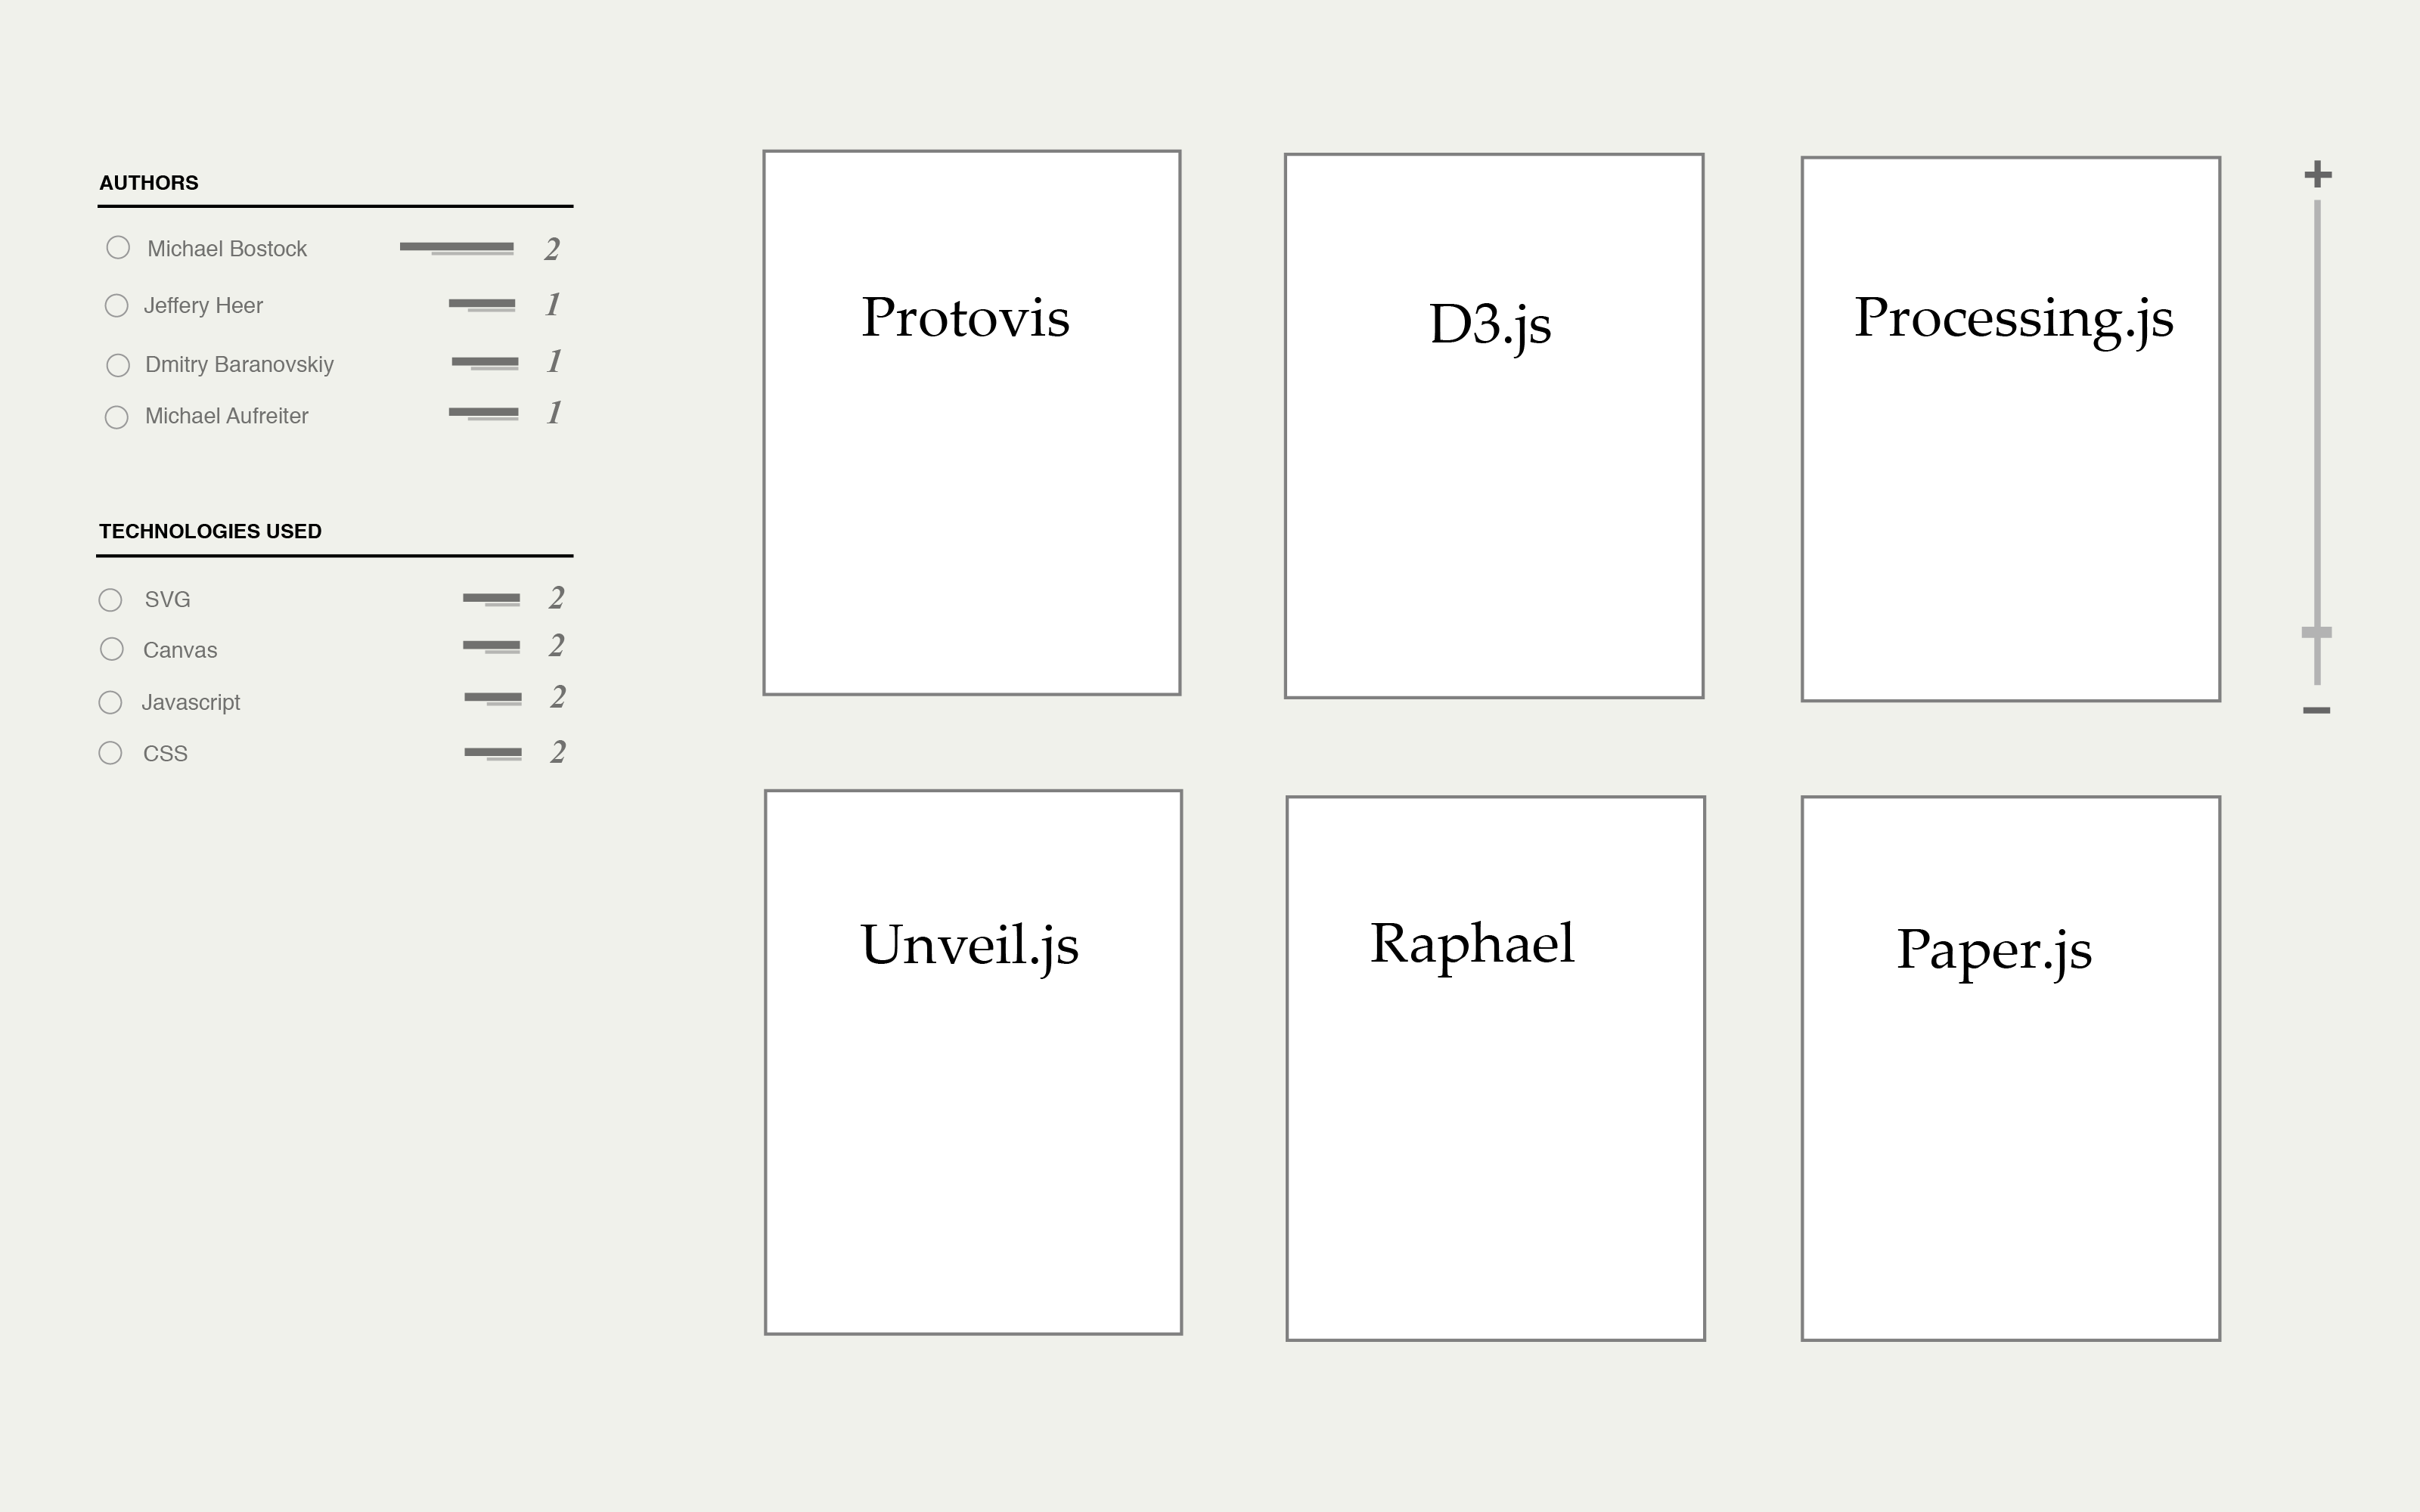
\includegraphics[width=1\textwidth]{doc_explorer/master_thesis_illustrations_2-01}
\caption{Overview: Shows all documents, along with a list of associated entities}
\label{fig:overview}
\end{figure}


\subsection{Zoom}
%%%-----------------------------------------------------------------------------

\begin{figure}
\centering
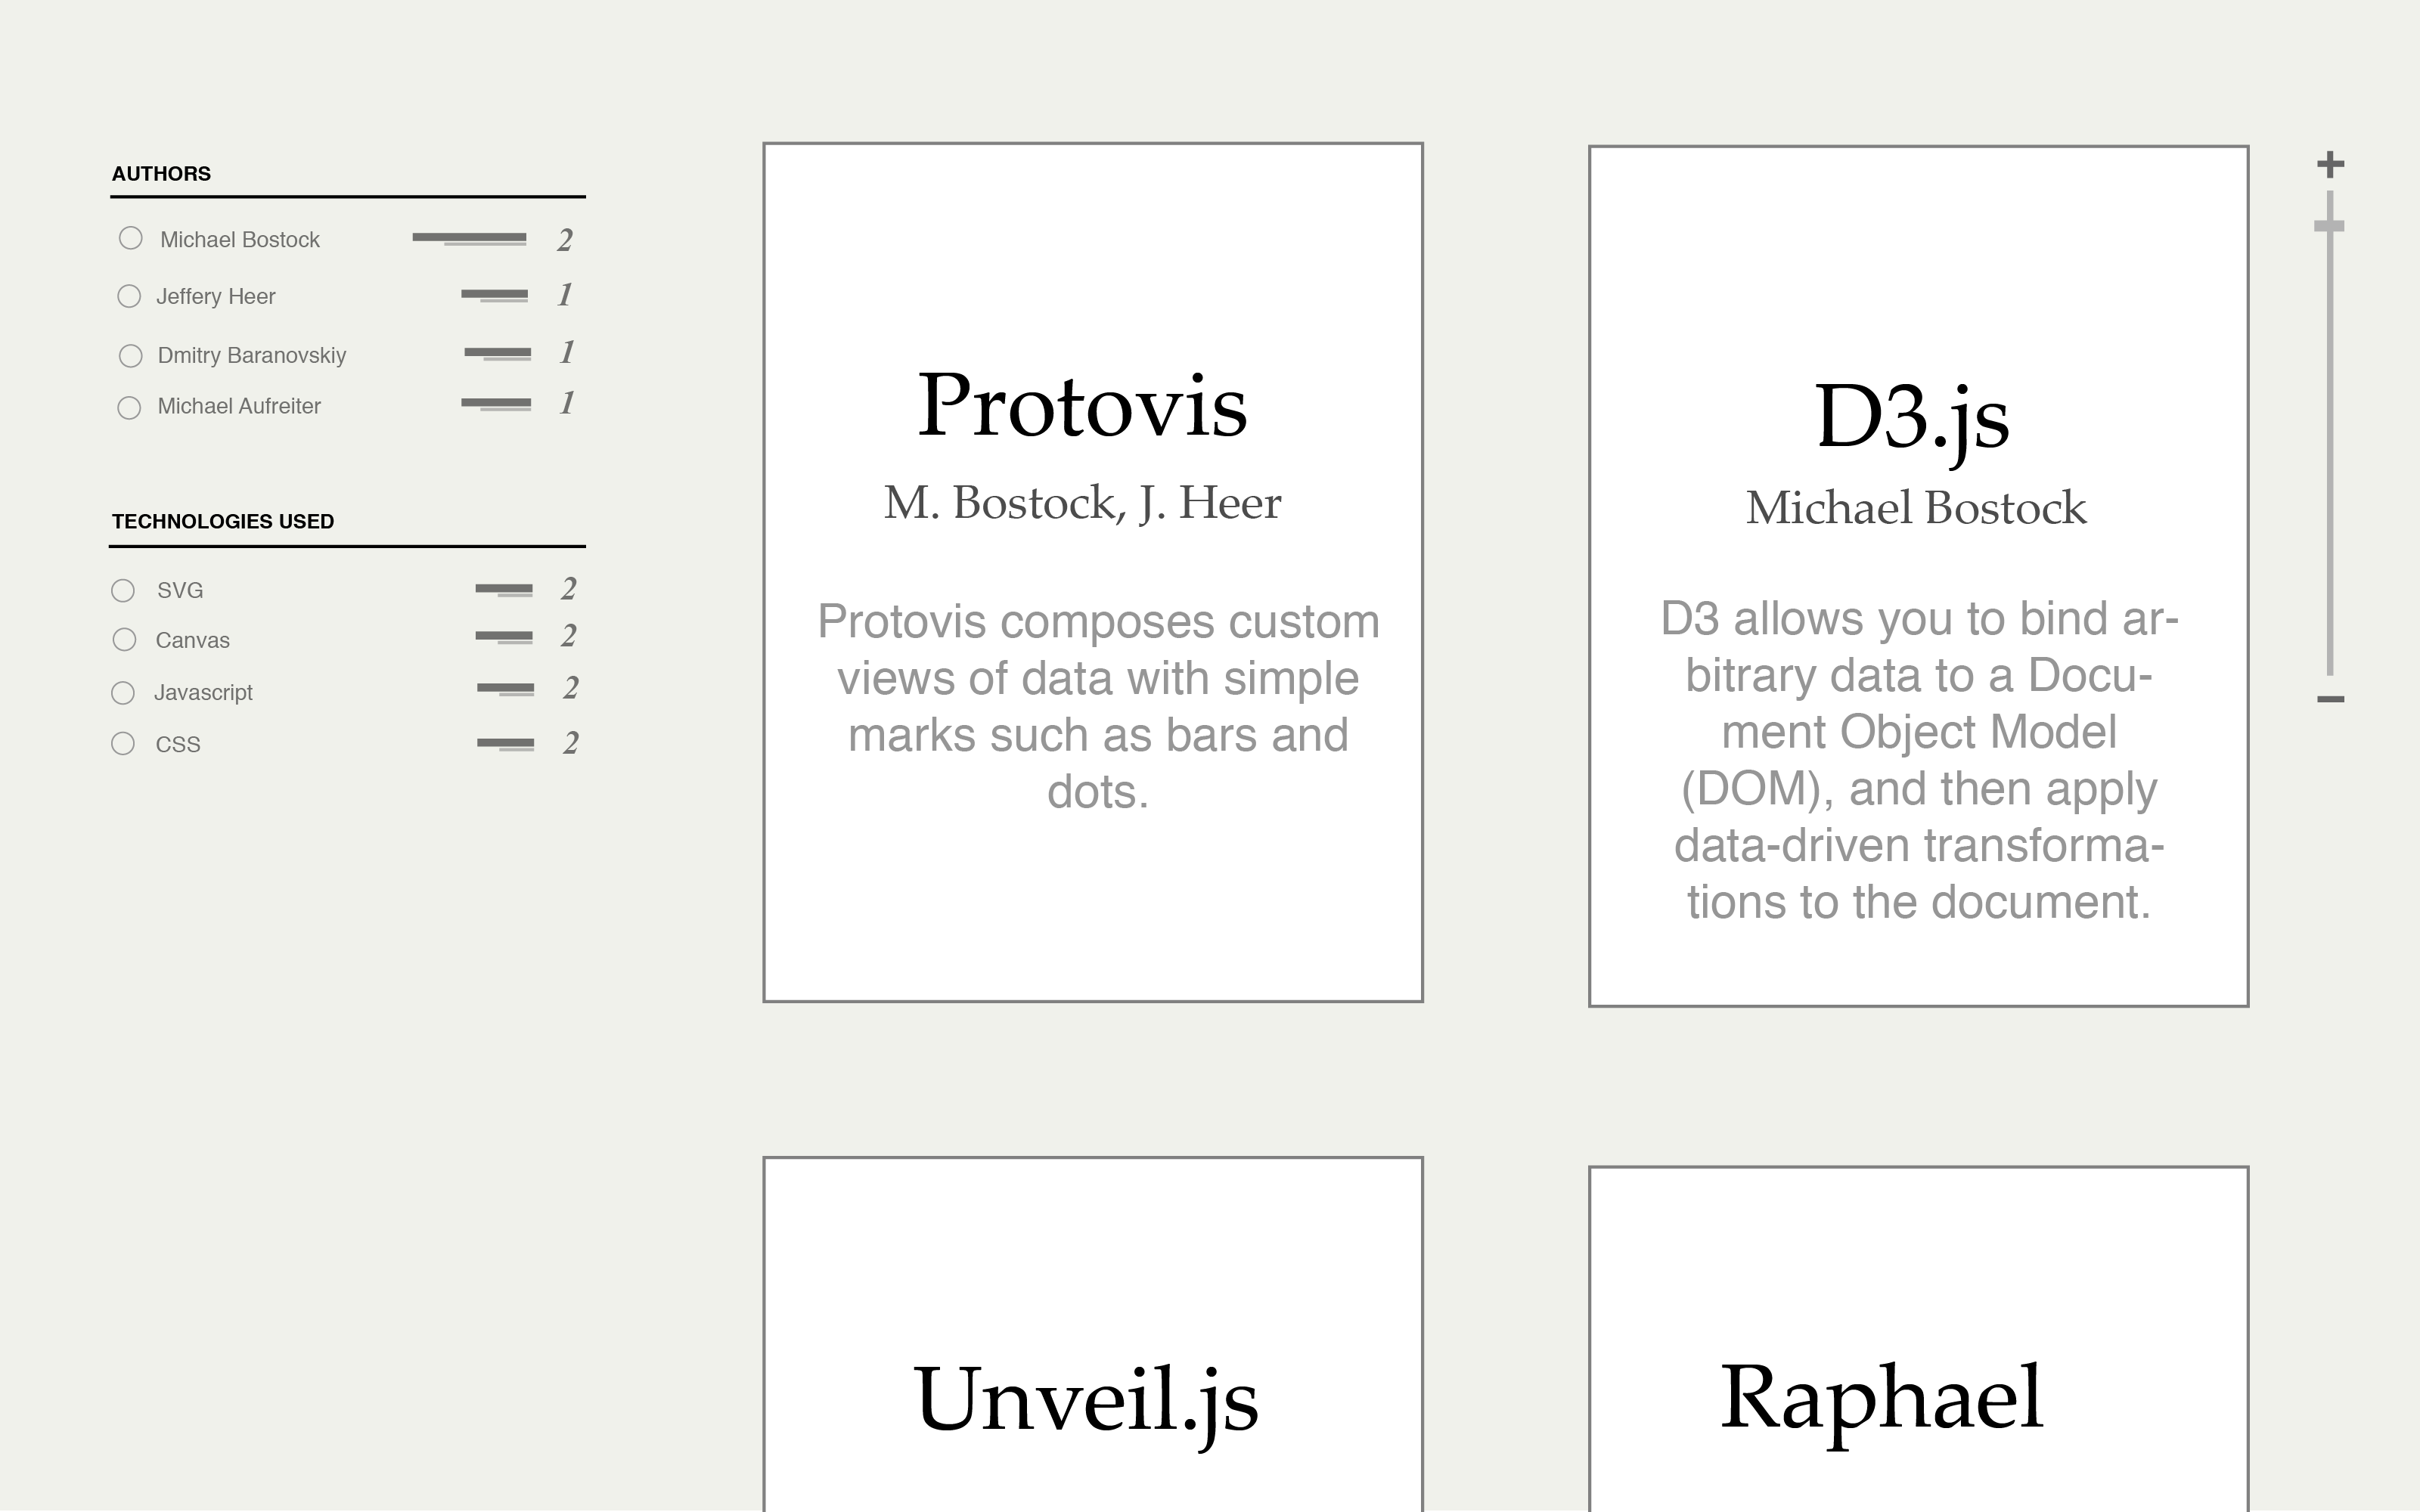
\includegraphics[width=1\textwidth]{doc_explorer/master_thesis_illustrations_2-02}
\caption{Zoom: Focus on the upper left area of the matrix plot}
\label{fig:zoom}
\end{figure}

A user might want to zoom in on items of interest. The user is likely to be interested in some portion of a collection. In order to focus on a particular area, control over the \emph{zoom focus} and \emph{zoom level} is needed. In Figure~\ref{fig:zoom} a user has zoomed into the upper left area. The increased zoom level unveils more details about the documents in focus, such as the author and a short abstract.

\subsection{Filter}
%%%-----------------------------------------------------------------------------

\begin{figure}
\centering
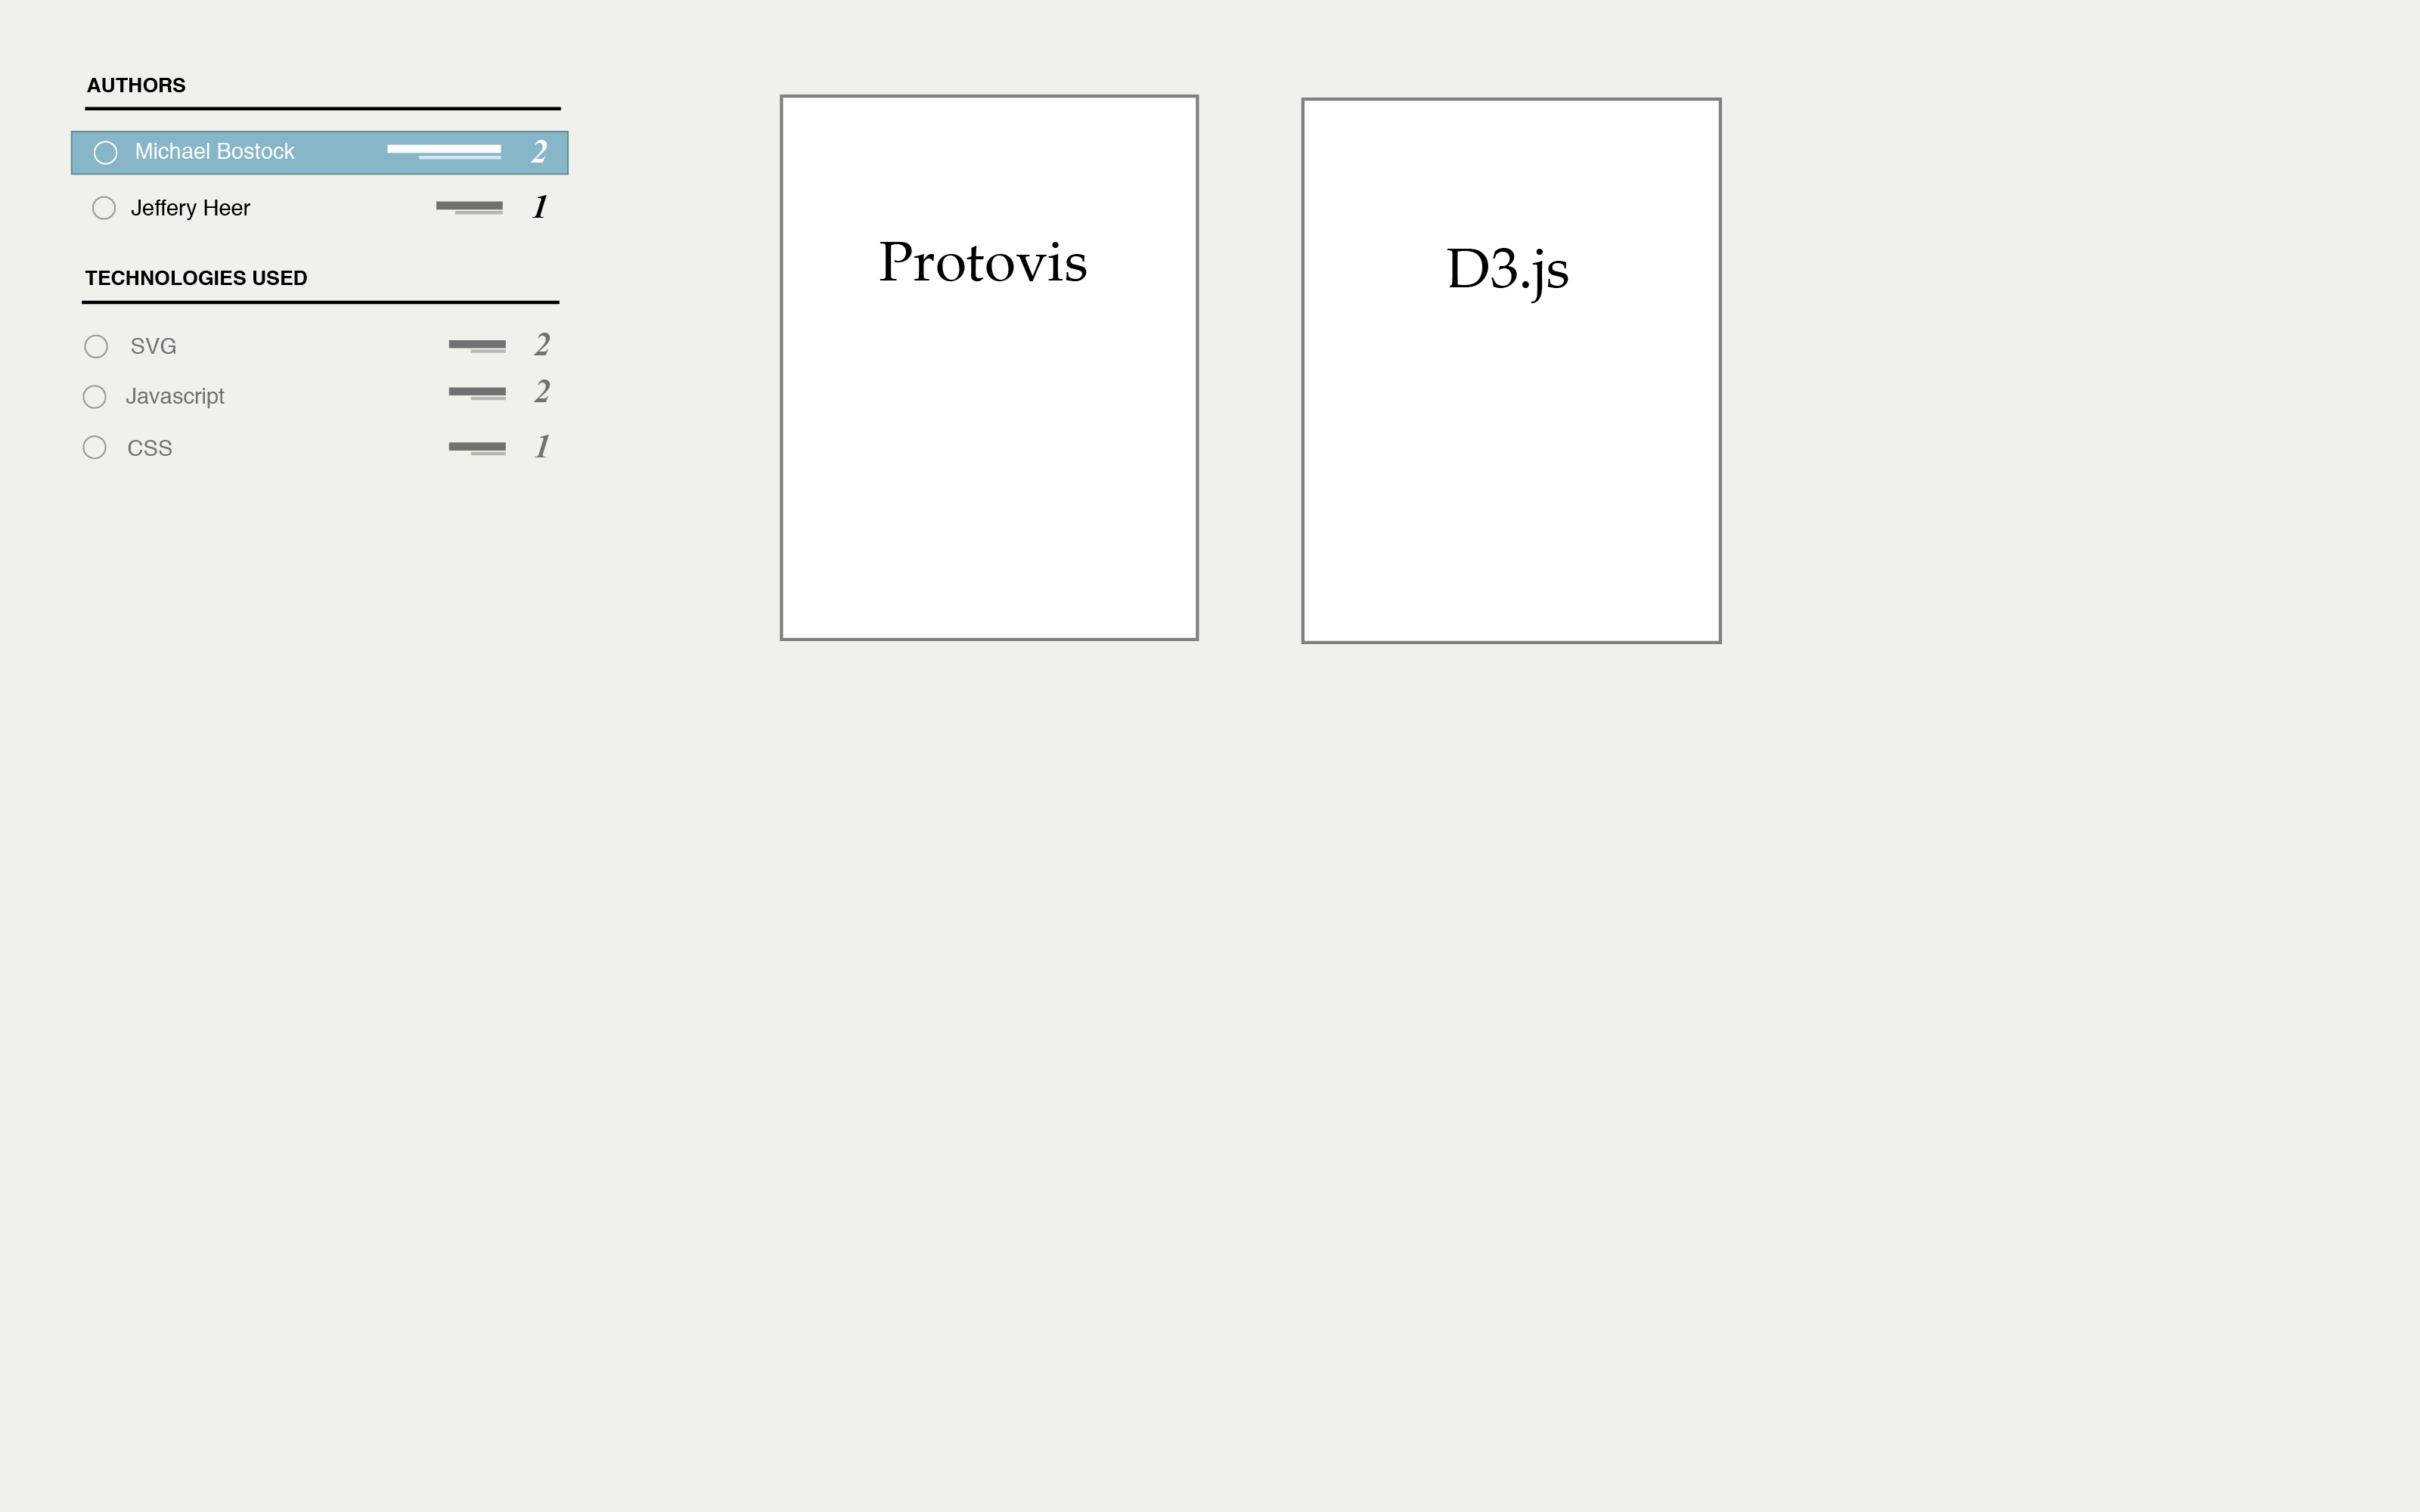
\includegraphics[width=1\textwidth]{doc_explorer/master_thesis_illustrations_2-05}
\caption{Filter: Filtering restricts the number of documents based on selected attributes}
\label{fig:filtering}
\end{figure}

Filtering allows the reduction of a dataset based on a user-defined set of criteria~\cite{Ahlberg92dynamicqueries}. Objects that do not match will no longer be included in the result. Filtering is an important tool for data exploration. It enables analysts to reveal facts that are not obvious when looking at the full dataset. Also implicit coherences can be discovered more easily. Thus, the quality of an interactive visualization depends to a high degree on the availability of extensive filtering options. Figure \ref{fig:filtering} shows a reduced set of documents based on a particular selection of entities.


\subsection{Details-on-demand}
%%%-----------------------------------------------------------------------------

\begin{figure}
\centering
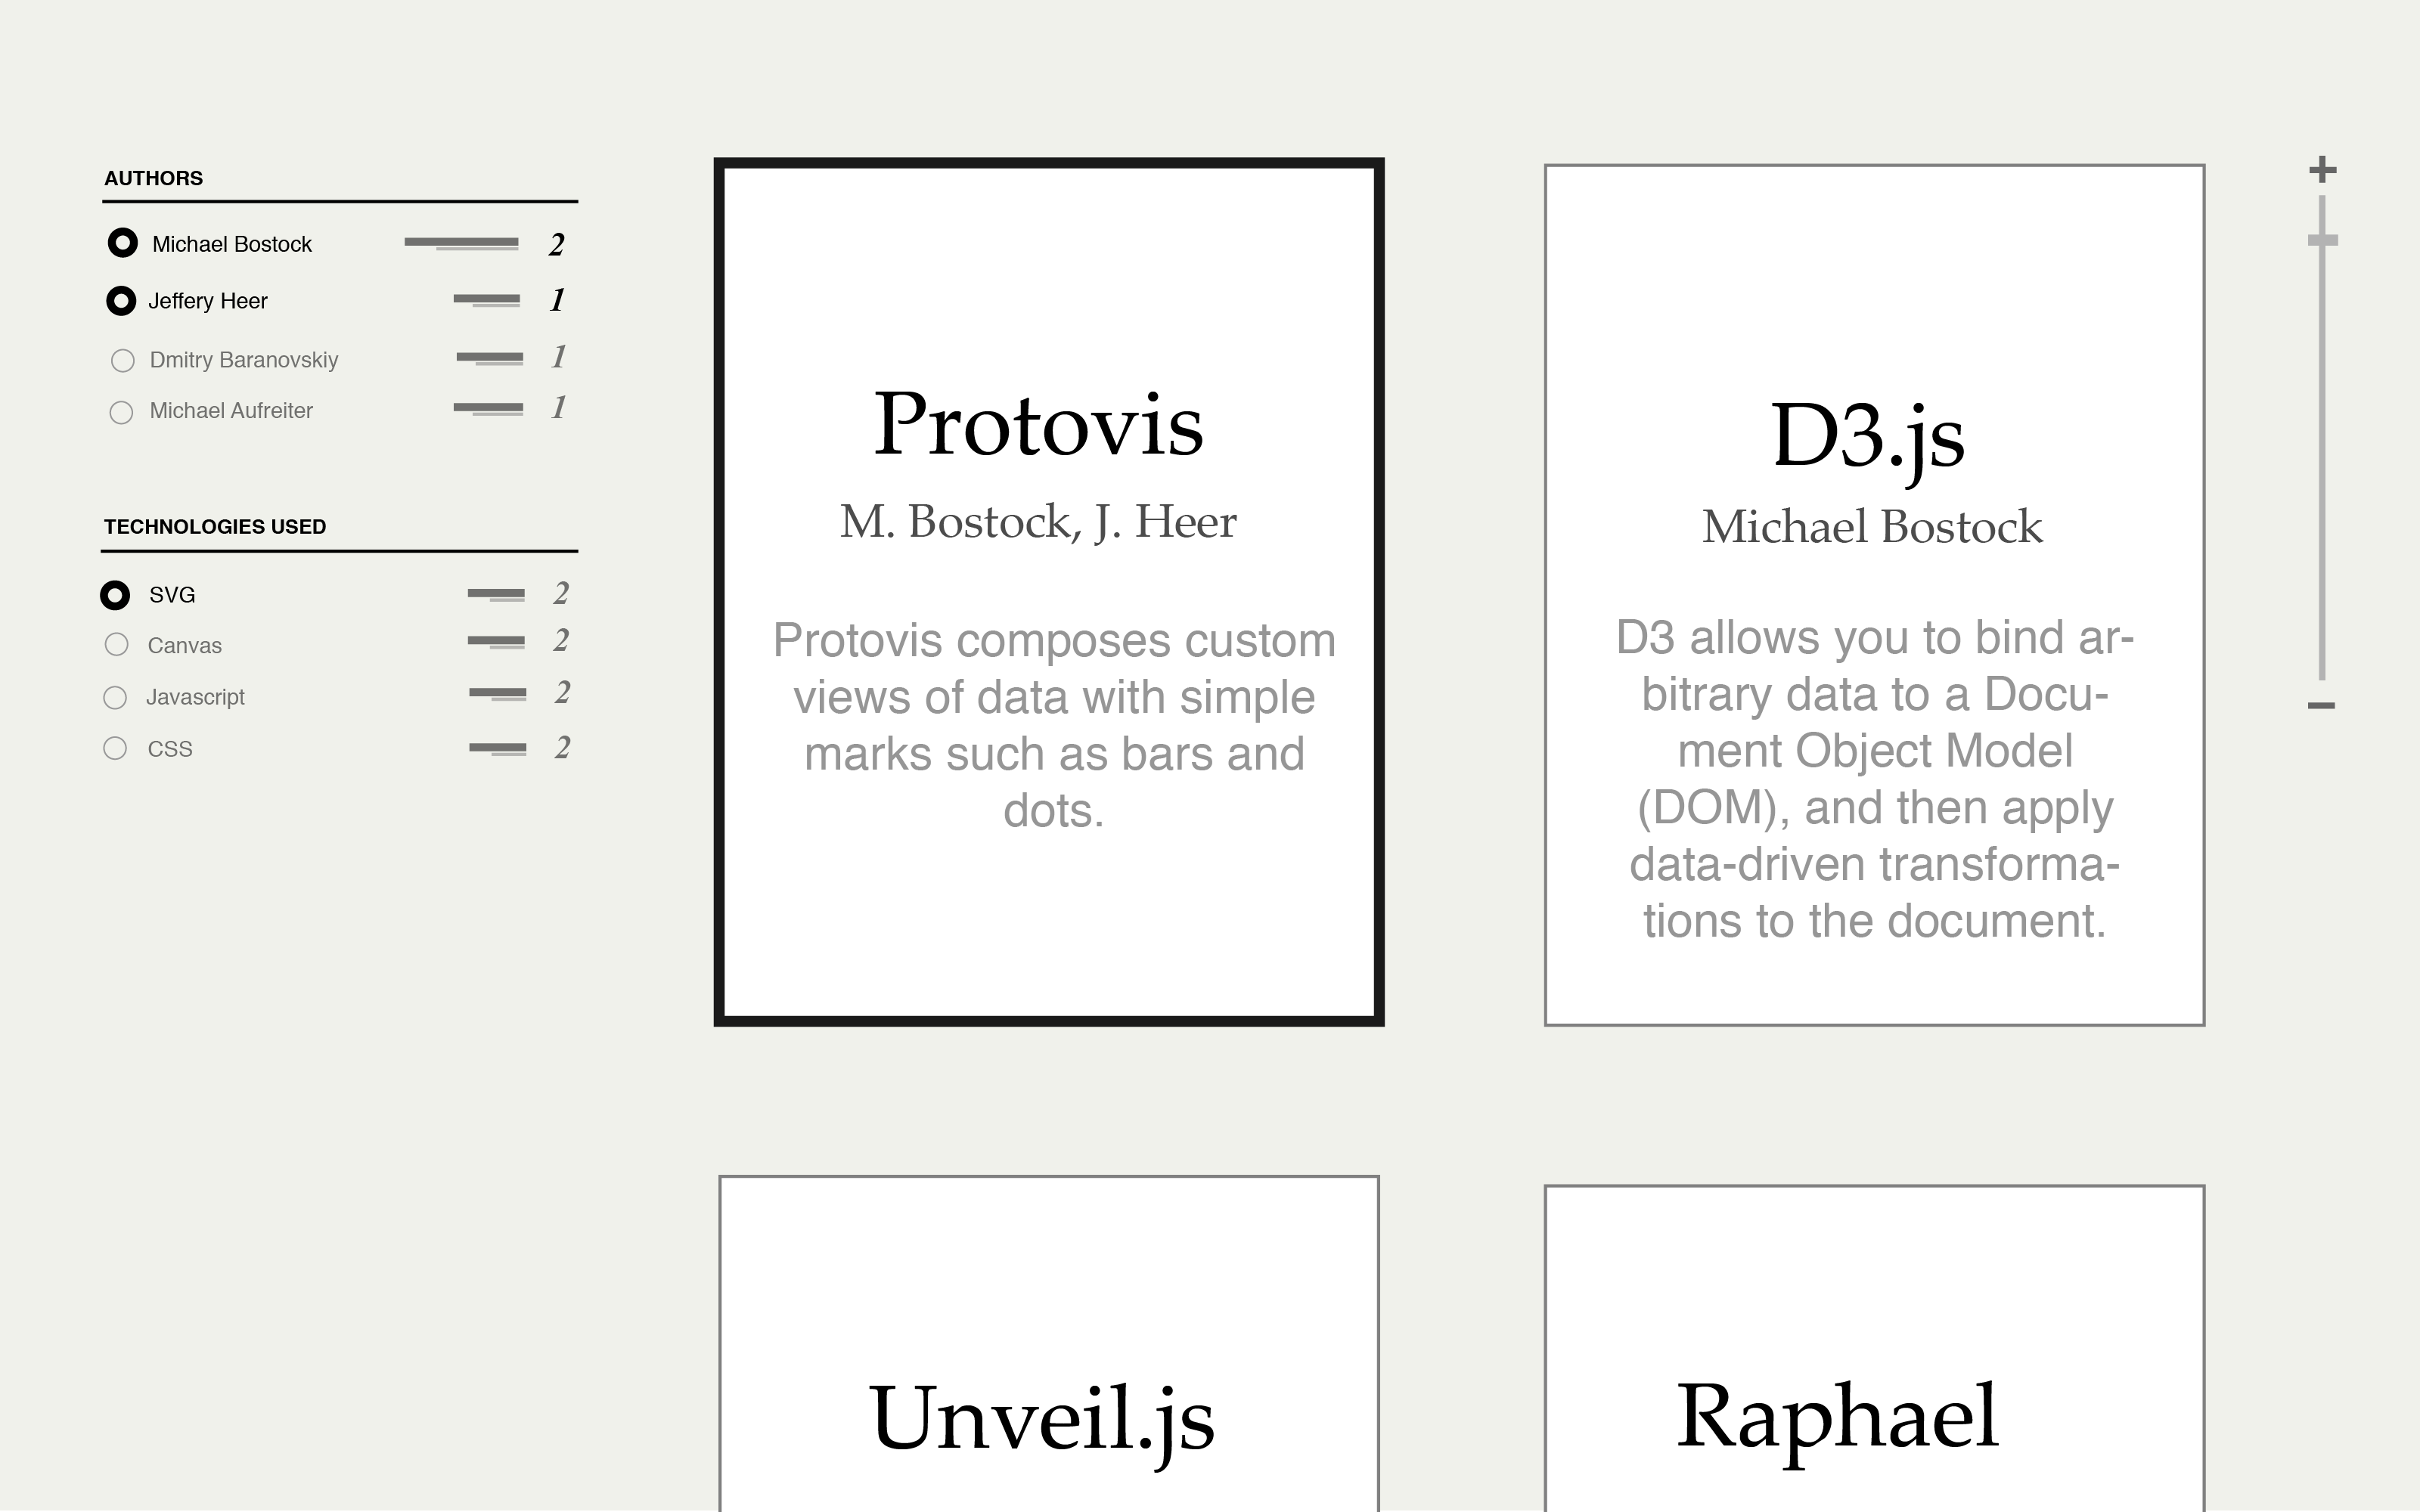
\includegraphics[width=1\textwidth]{doc_explorer/master_thesis_illustrations_2-03}
\caption{Detail-on-demand: For a certain object additional details, like associated entities are displayed}
\label{fig:detail}
\end{figure}

Users usually want to find out details for a selected object. This is usually done by providing a popup window containing the values of each attribute~\cite{shneiderman96eyes}. However, there are other options such as displaying contextual information based on the currently selected item, as shown in Figure~\ref{fig:detail}.


\subsection{Relate}
%%%-----------------------------------------------------------------------------

Viewing relationships between data items is also an important task. Based on an attribute selection, as shown in Figure \ref{fig:relate}, users can find out which documents are associated with both ``Michael Bostock'' and ``Jeffery Heer''. Color coding is used to connect documents with concrete attributes. In addition to that, size is used to encode relevance. Documents that contain all selected entities are displayed at maximum size while others, which only match one entity, appear smaller. Documents that do not match are greyed out.

\begin{figure}
\centering
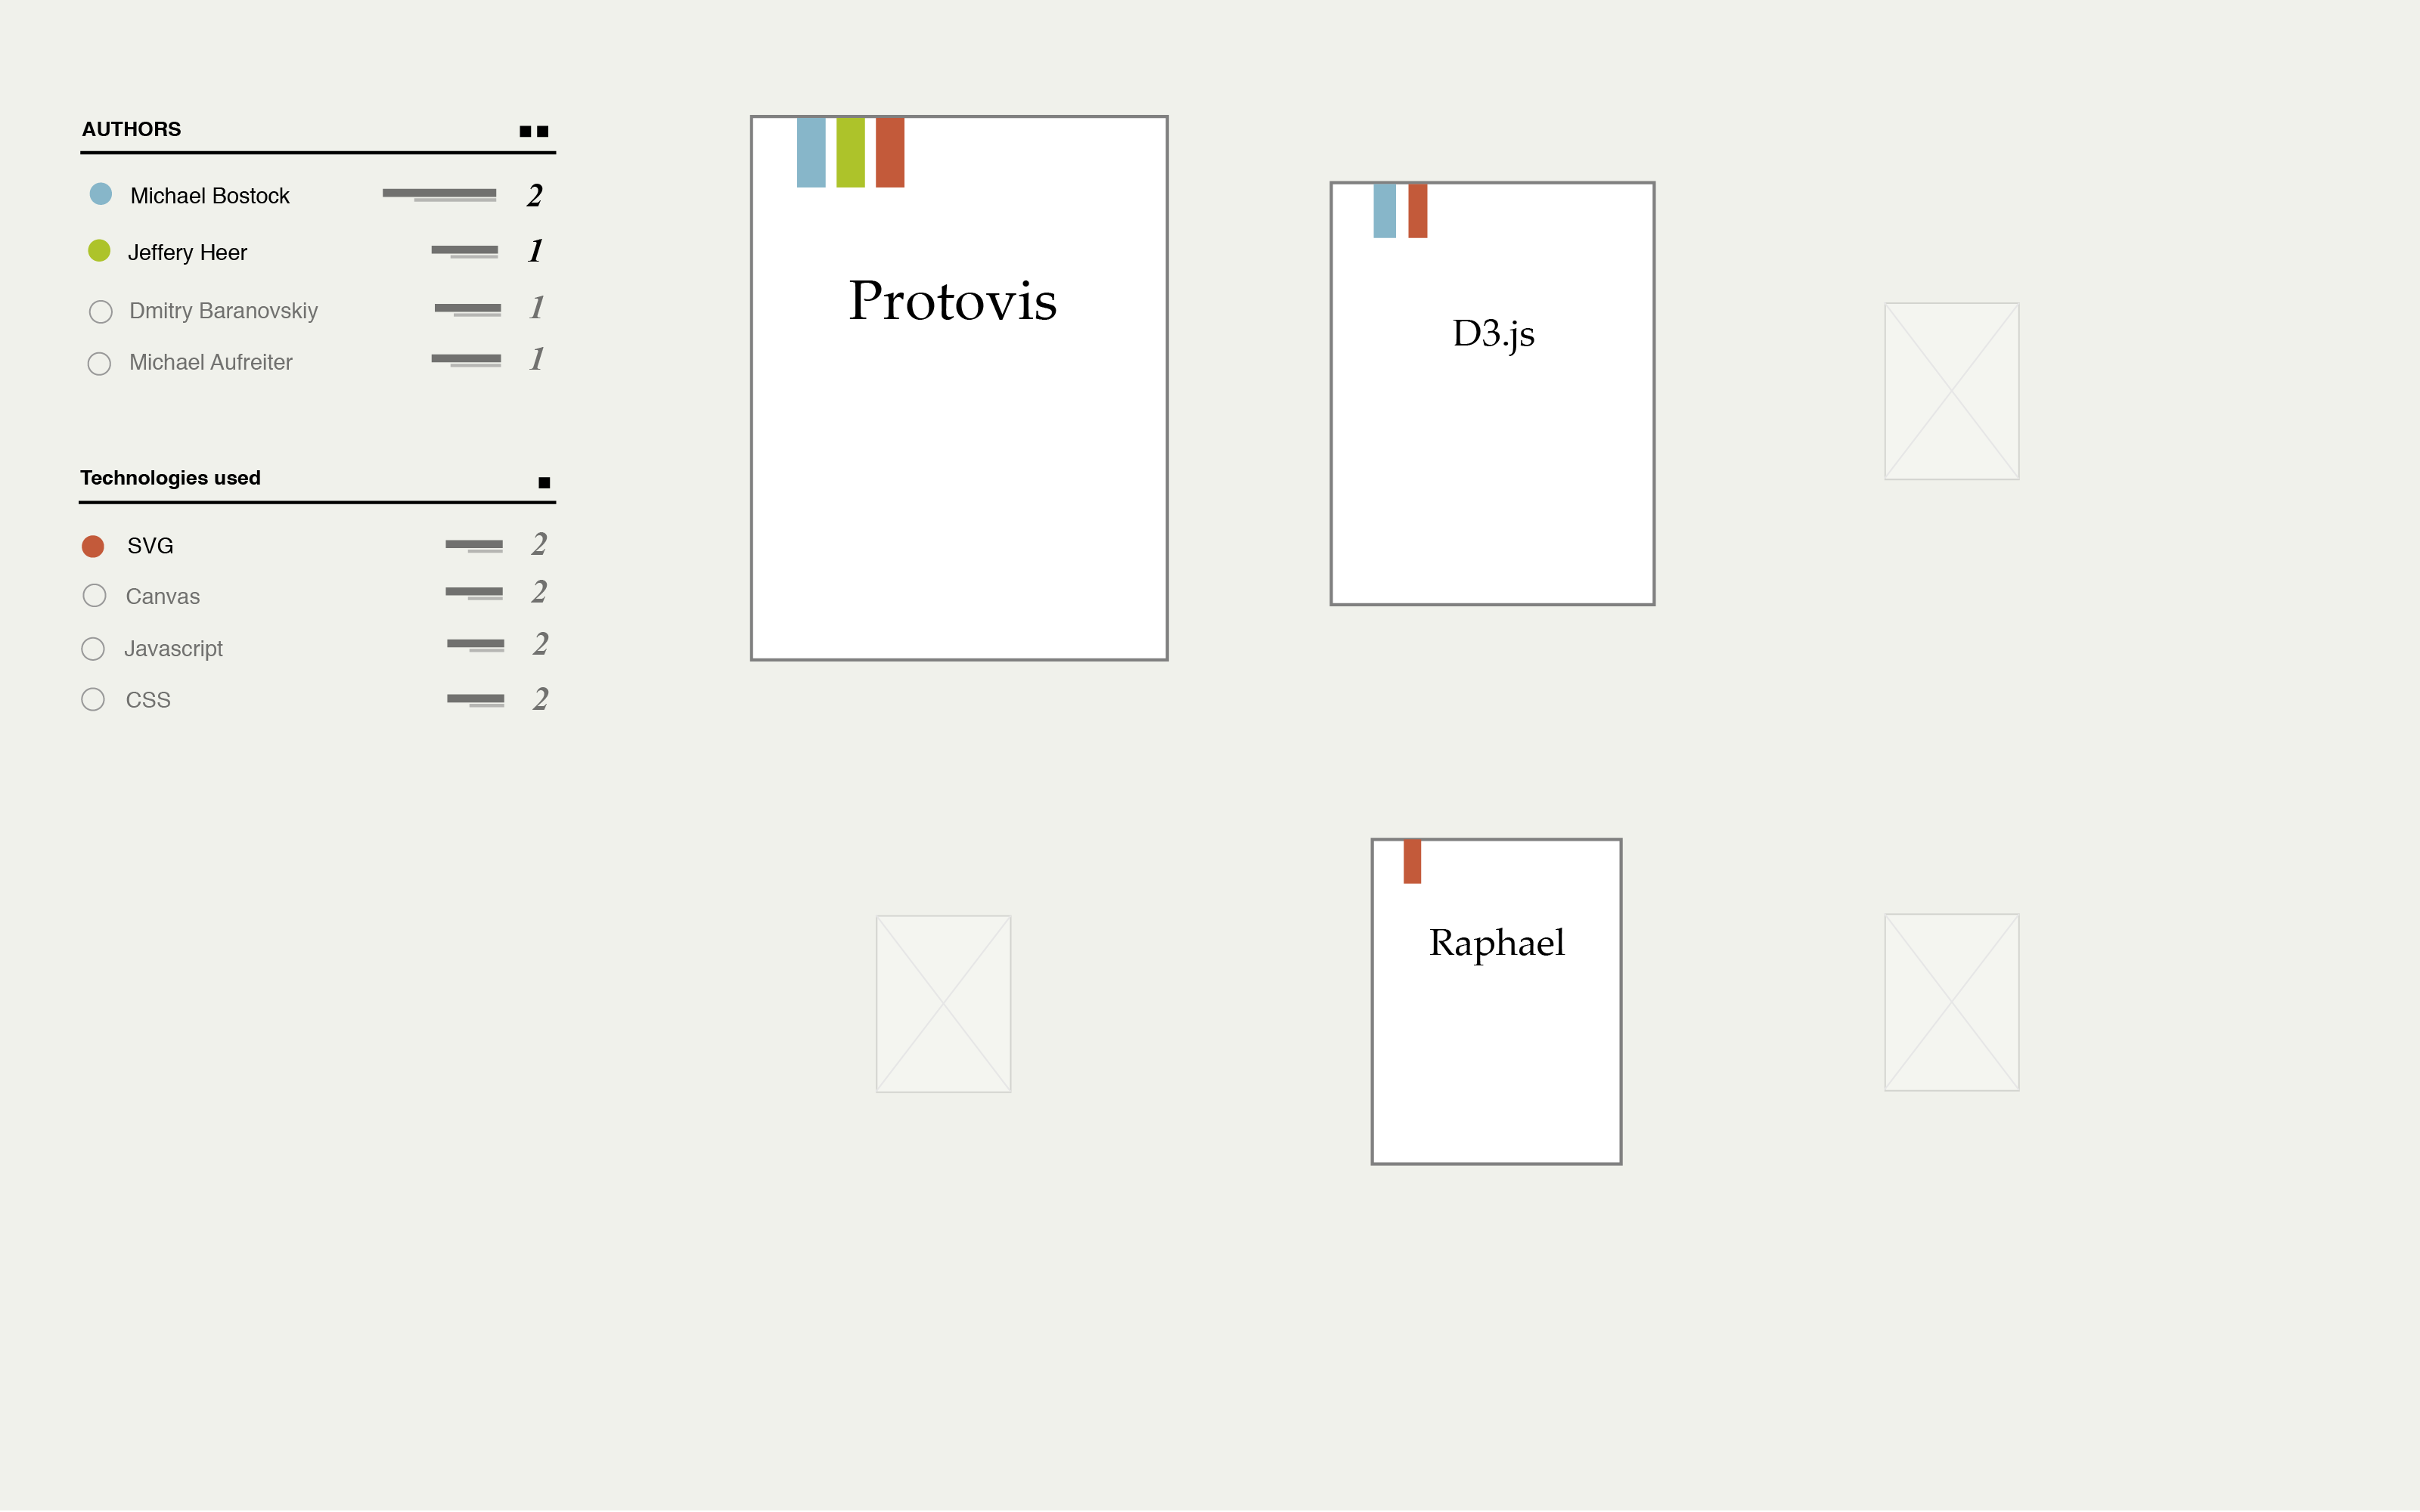
\includegraphics[width=1\textwidth]{doc_explorer/master_thesis_illustrations_2-04}
\caption{Relate: Based on a selection of entities relationships among documents are revealed}
\label{fig:relate}
\end{figure}


\subsection{History}
%%%-----------------------------------------------------------------------------

It is useful to keep a history of actions performed by the user to support \emph{undo}, \emph{replay} and \emph{progressive refinement}. Information Exploration is a task which involves many steps. In order to support the user, it should be possible to retrace the steps performed~\cite{shneiderman96eyes}.


\subsection{Extract}
%%%-----------------------------------------------------------------------------

Based on the current application state, users should be able to store a snapshot of the current context. Later they are either able to restore that context or to share their explorations with others. In a web-based context shareable URL's can be used for state extraction, which is called \emph{View Sharing}~\cite{clark91}.


\section{Data Types}
%%%-----------------------------------------------------------------------------

The following classification by \emph{Data Type}, adapted from Shneiderman \cite{shneiderman96eyes}, is not meant to be seen as strict, but can be helpful to organize visual designs mentally into classes. The \emph{Data Types} described are closely related to how an item of a collection suits a corresponding graphical representation. Based on the explanations of Shneiderman, user problems as well as possible graphical representations are identified for each type.


\subsection{1-dimensional}
%%%-----------------------------------------------------------------------------

% \begin{figure}
% \centering
% 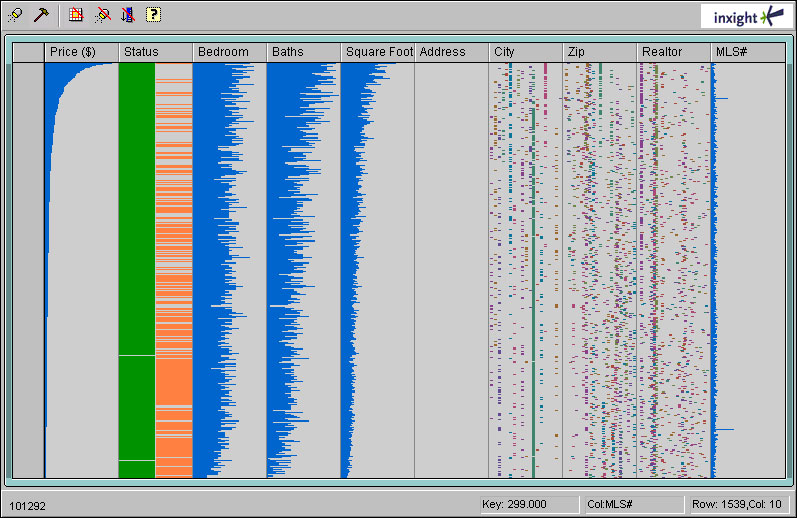
\includegraphics[width=1\textwidth]{tablelens}
% \caption{Table Lens}
% \label{fig:tablelens}
% \end{figure}

1-dimensional data refers to \emph{linear} data types which are organized in a \emph{sequential} manner, such as documents, program source code or an alphabetical list of names~\cite{shneiderman96eyes}. Users usually want to access global information about the characteristics of the data they are viewing as well as how a particular element in the list compares to others. Sometimes users might want to search for specific results within the full dataset based on user defined criteria. This is commonly solved by applying methods for \emph{scrolling} to pick up desired elements. To improve the effectiveness of navigation, compact visual presentations are used, which encode certain properties (such as the number of characters of a line) to represent individual items in the collection.


\SuperPar User problems:

\begin{itemize}
\item Find the total number of items
\item Find items, e.g. a line in a document, that match particular attributes (e.g. if the line is a section)
\end{itemize}


\begin{figure}
\centering
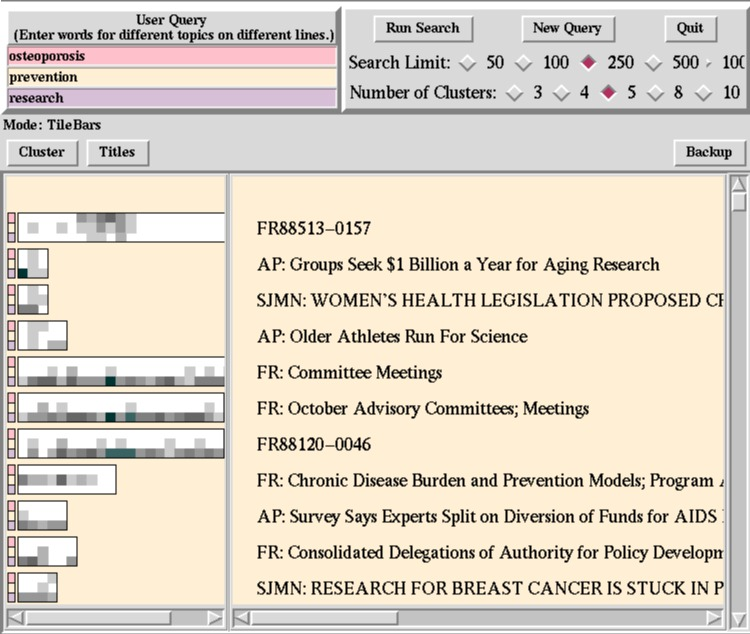
\includegraphics[width=1\textwidth]{tilebars}
\caption{Tilebars visualizing the output of a query to a medical database with three terms: osteoporosis, prevention and research. While Tilebars on the left show relationships between those terms, corresponding documents appear on the right.}
\label{fig:tilebars}
\end{figure}

\SuperPar Examples:

\begin{itemize}
\item \textbf{Tilebars}~\cite{Hearst95tilebars} encode contents of documents using bars. As shown in Figure~\ref{fig:tilebars}, rectangle shading is used to indicate absence or presence of topics within a document.
\item \textbf{The Table Lens}~\cite{tablelens97} is an example for a Bifocal Display~\cite{Spence82} that shows detailed information in focus and less information in the surrounding area.
\end{itemize}


\subsection{2-dimensional}
%%%-----------------------------------------------------------------------------

Planar or map data, such as geographic maps, floor plans or computer chip designs are examples for 2-dimensional data. It is characterized by items in a collection that cover some part of the total area available. A dataset can be considered 2-dimensional if questions about \emph{direction}, \emph{location}, \emph{size} and \emph{distance} can be answered. For a collection of countries including geo information, possible questions could be: How close is Prague to Vienna? How big is Prague compared to Vienna? 2-dimensional data contains a number of attributes that will be used in the visual environment. Examples for such attributes are longitude and latitude, width and height, etc. In reality, all data visualization environments are displayed on a 2D surface, which sometimes leads to confusion regarding classifying data as 2-dimensional.

\begin{figure}
\centering
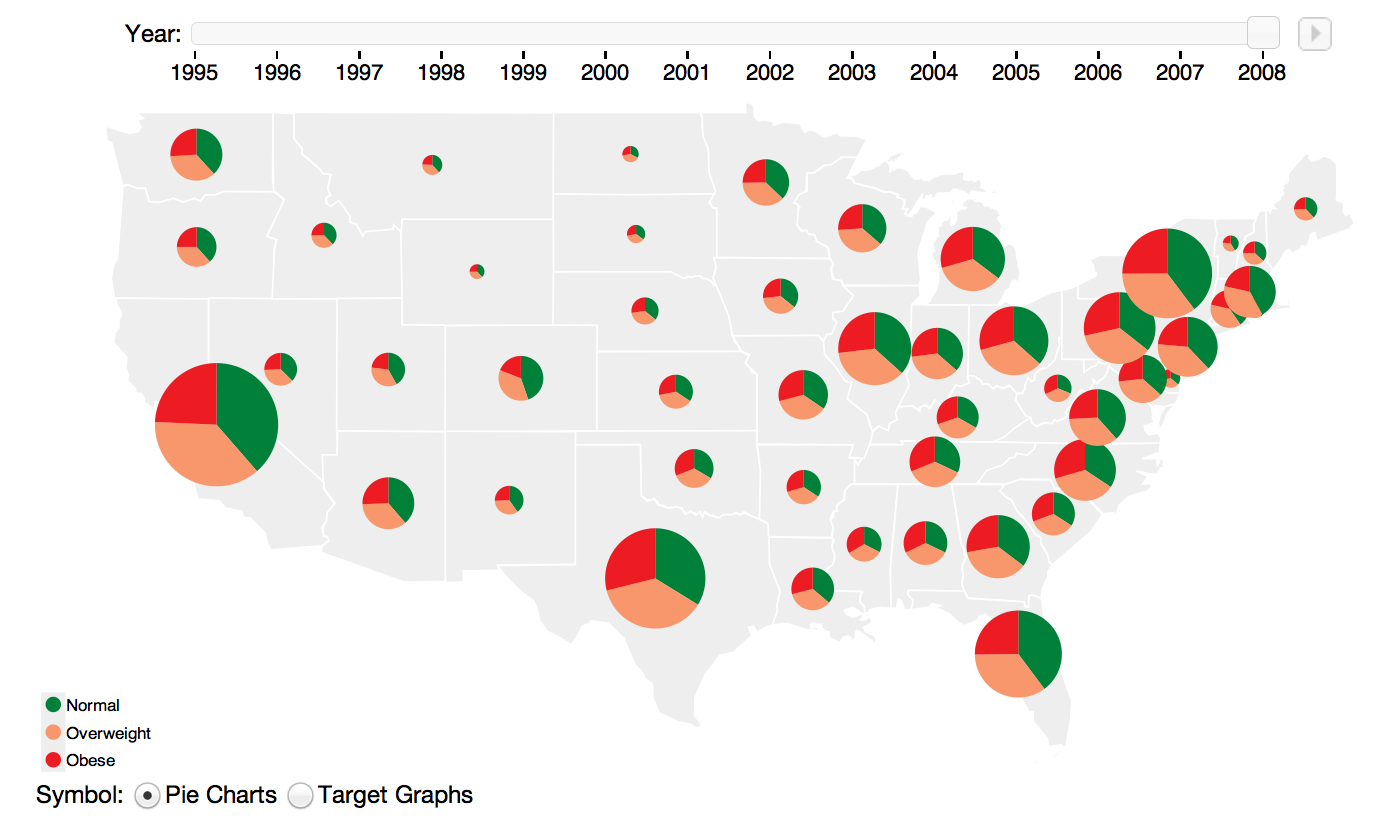
\includegraphics[width=1\textwidth]{map}
\caption{Graduated Symbol Map of Obesity in the U.S., 2008}
\label{fig:map}
\end{figure}

\SuperPar User Problems:

\begin{itemize}
\item Find adjacent items
\item Containment of one item by another
\item Paths between items
\end{itemize}

\SuperPar Examples:

\begin{itemize}
\item \textbf{Graduated Symbol Maps}, as shown in Figure~\ref{fig:map}, place symbols over an underlying map that are used to encode a variable associated with a geographic region~\cite{VisualizationZoo:2010}.
\item \textbf{Cartograms} distort the shape of a geographic region, so that the area directly encodes an associated data variable. Figure~\ref{fig:cartogram} shows a Dorling Cartogram, which represents each geographic region with a sized circle~\cite{VisualizationZoo:2010}.
\end{itemize}

\begin{figure}
\centering
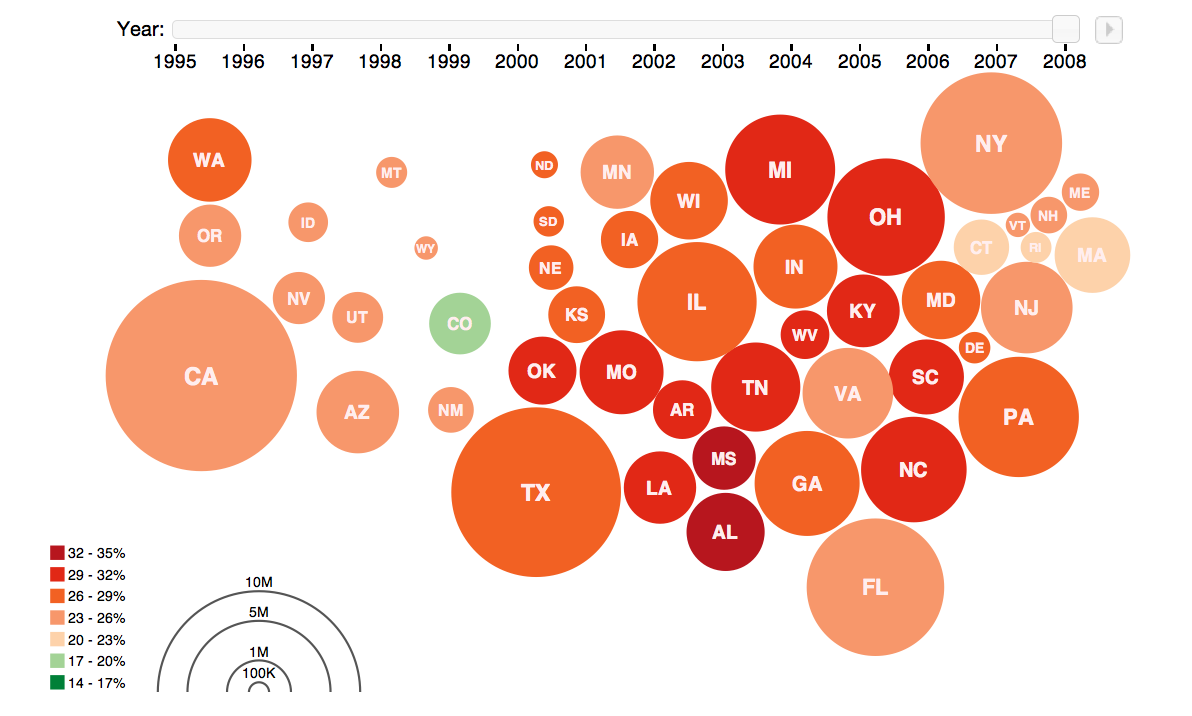
\includegraphics[width=1\textwidth]{cartogram}
\caption{Dorling Cartogram of Obesity in the U.S., 2008}
\label{fig:cartogram}
\end{figure}



\subsection{3-dimensional}
%%%-----------------------------------------------------------------------------

\begin{figure}
\centering
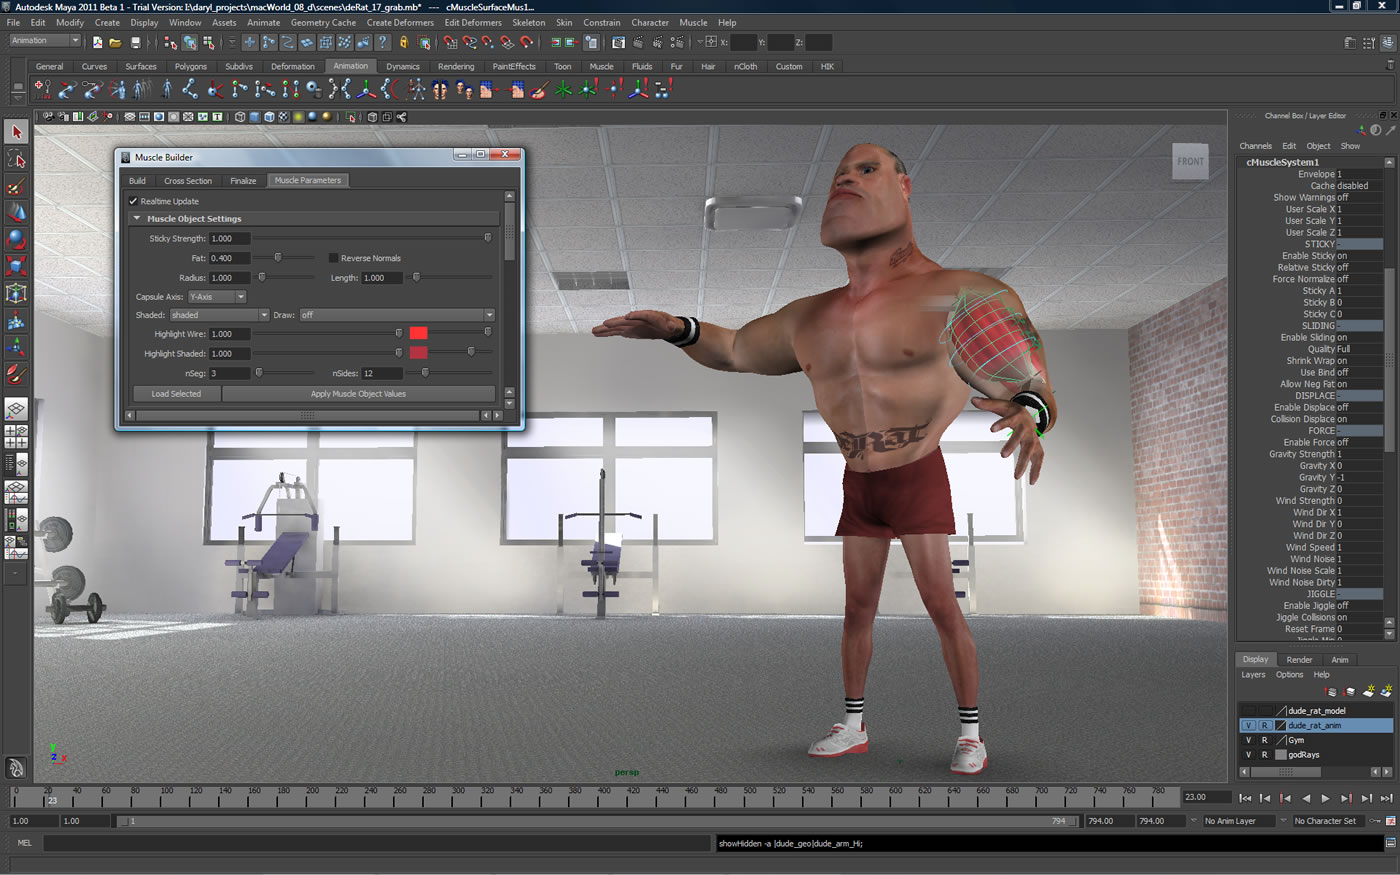
\includegraphics[width=1\textwidth]{maya}
\caption{Autodesk Maya utilized for character animation}
\label{fig:maya}
\end{figure}

3-dimensional data involves real-world objects like landscapes, the human body or buildings. Such objects are typically composed of lower level objects, involving volume and complex relationships between each other~\cite{shneiderman96eyes}. Computer-assisted design systems (CAD) for architects or 3D animation software are designed to handle 3-dimensional relationships. While 3D computer graphics and computer assisted design are employed frequently, Information Visualization in three dimensions is still novel. 3D representation in the context of Information Visualization should be applied with care. If a dataset can effectively be represented in two dimensions, plotting them in 3D space does not add any value. What the presenter creates here has been called ``chart chunk'' by Edward Tufte~\cite{tufte09}.


\begin{figure}
\centering
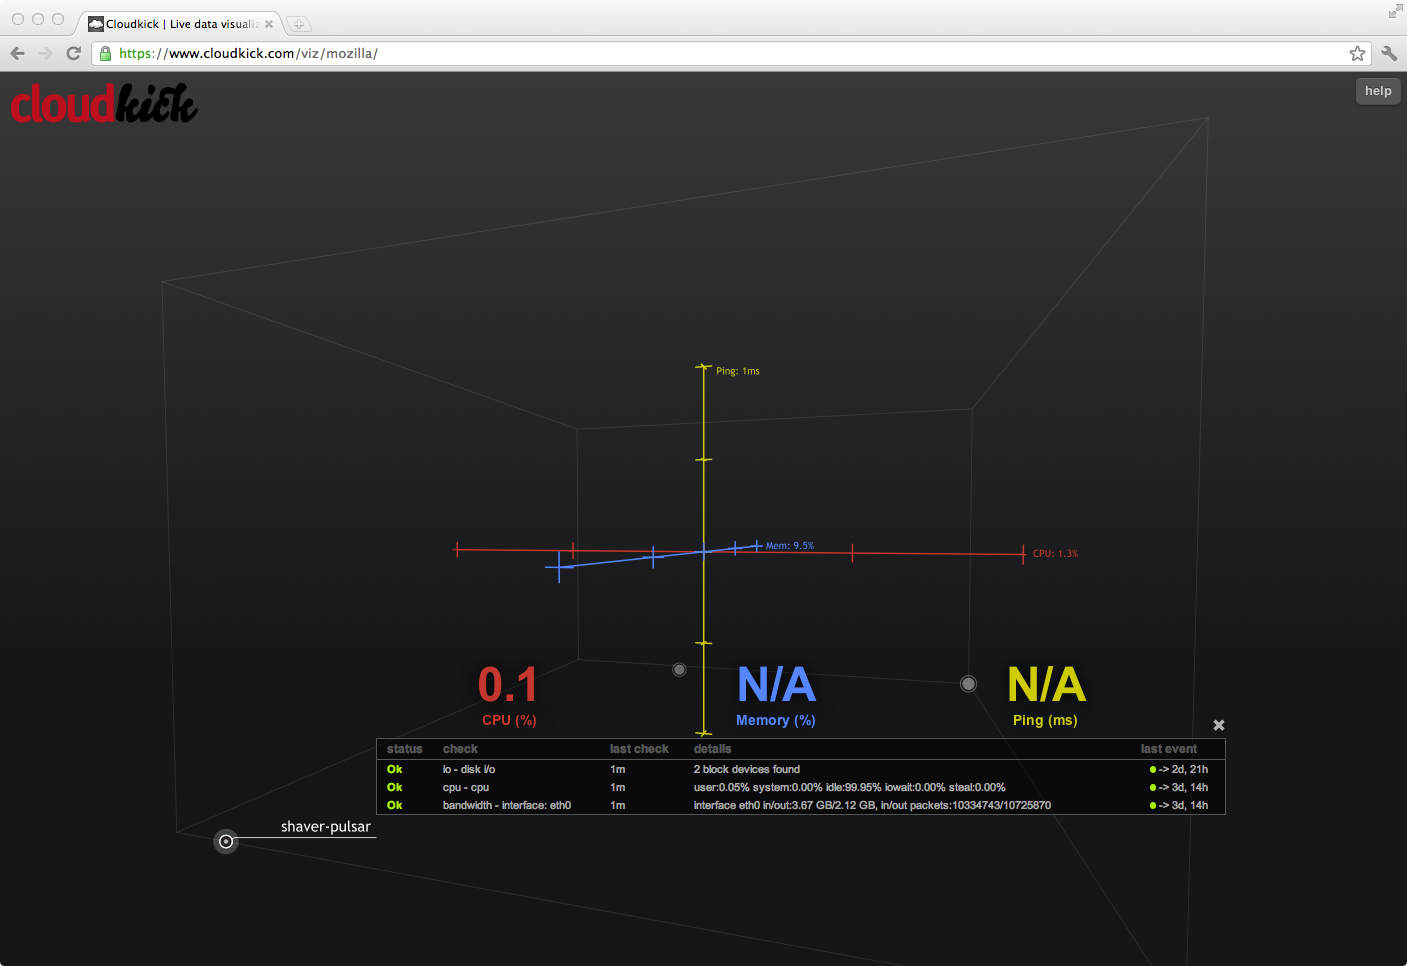
\includegraphics[width=1\textwidth]{cloudkick}
\caption{Cloudkick Vis: Monitored Servers of a cloud infrastructure are plotted in 3-dimensional space, according to performance metrics like CPU usage, Memory usage, and Ping latency.}
\label{fig:cloudkick}
\end{figure}


\SuperPar User Problems:

\begin{itemize}
\item Find adjacent items
\item Understanding the current position and orientation
\item Detecting occlusion
\item Containment issues
\end{itemize}


\SuperPar Examples:

\begin{itemize}
\item \textbf{Autodesk Maya}\footnote{http://usa.autodesk.com/maya}, as shown in Figure~\ref{fig:maya}, is a 3D composition software that provides tools for \emph{animation}, \emph{modeling}, \emph{visual effects} and \emph{rendering}.
\item \textbf{Cloudkick Vis}\footnote{https://www.cloudkick.com/viz/mozilla/} (Figure~\ref{fig:cloudkick}) is a visual server monitoring workspace that displays server status information in realtime.
\end{itemize}


\subsection{Temporal}
%%%-----------------------------------------------------------------------------

Temporal data involves values changing over time and is one of the most common forms of recorded data. Time-varying phenomena are important to many domains such as finance, science and public policy. Time series data often needs to be compared simultaneously and demands suitable visualizations. Shneiderman~\cite{shneiderman96eyes} draws a distinction to 1-dimensional data as soon as data items have a start and finish time (which may overlap).


\begin{figure}
\centering
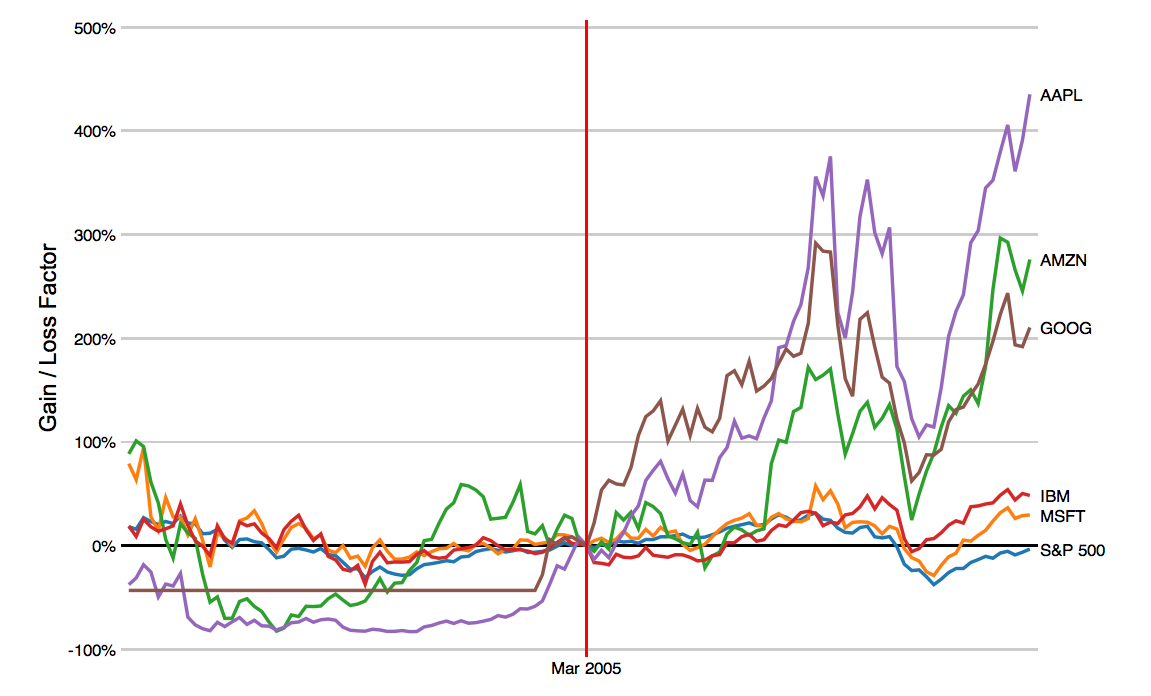
\includegraphics[width=1\textwidth]{timeseries}
\caption{Index Chart of Selected Technology Stocks, 2000-2010}
\label{fig:timeseries}
\end{figure}

\SuperPar User Problems:

\begin{itemize}
\item Get a chronologic overview about events that happened
\item Find events during a specific time period
\end{itemize}

\SuperPar Examples:

\begin{itemize}
\item \textbf{Index Charts} are used to display relative changes over time~\cite{VisualizationZoo:2010}. Figure~\ref{fig:timeseries} shows the gain/loss factors of selected technology stocks.
\item \textbf{Stacked Graphs} show time series as an aggregation by stacking area charts on top of each other~\cite{VisualizationZoo:2010}. As shown in Figure~\ref{fig:stackedgraph}, the result is a visual summation of time-series values.
\end{itemize}


\begin{figure}
\centering
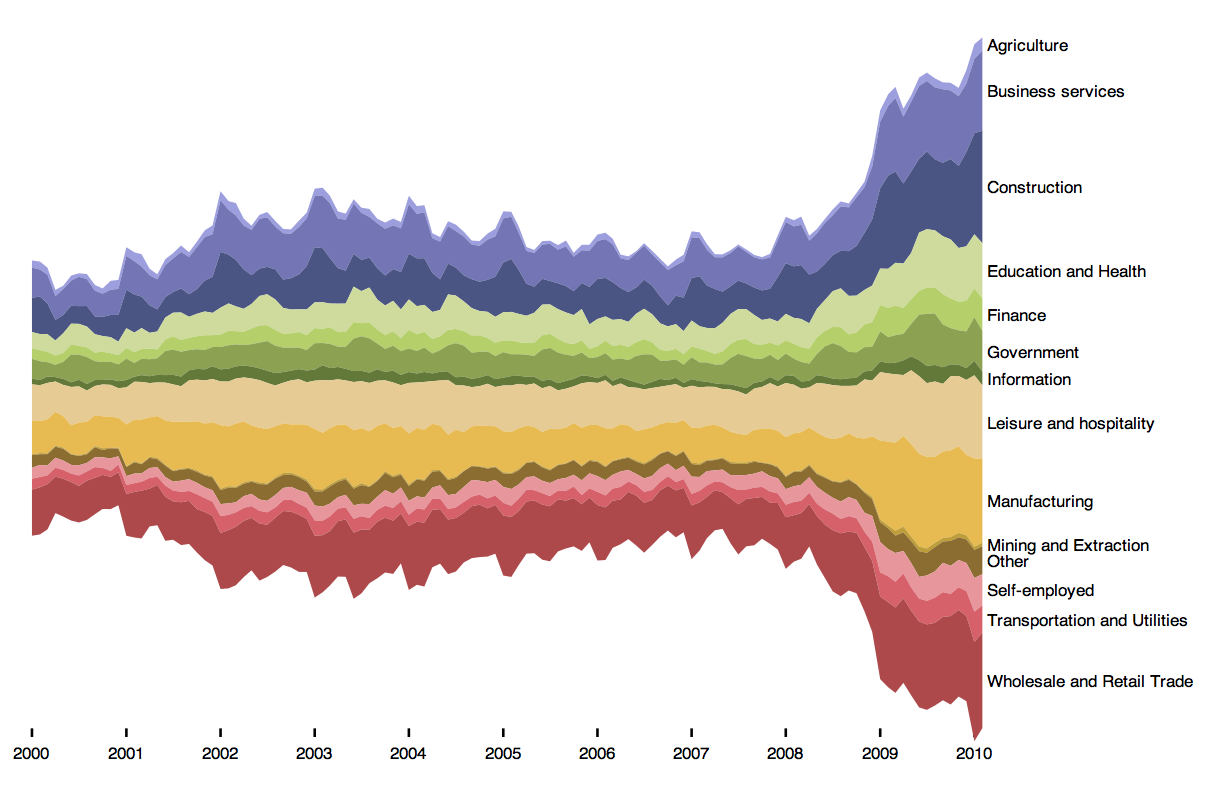
\includegraphics[width=1\textwidth]{stackedgraph}
\caption{Stacked Graph of Unemployment U.S. Workers by Industry, 2000-2010}
\label{fig:stackedgraph}
\end{figure}


\subsection{Multi-dimensional}
%%%-----------------------------------------------------------------------------

\begin{figure}
\centering
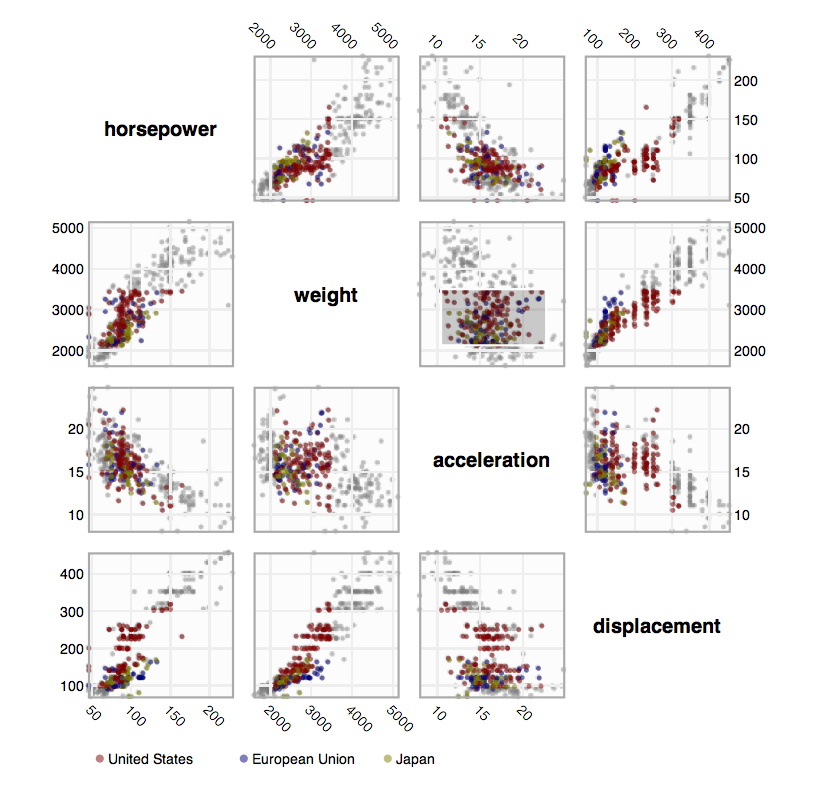
\includegraphics[width=1\textwidth]{scatterplot-matrix}
\caption{Scatter Plot Matrix of Automobile Data}
\label{fig:scatterplot-matrix}
\end{figure}

Multi-dimensional data, characterized by items with n-attributes, occurs frequently and is hard to represent, since it is difficult to picture data mentally in more than three dimensions. An example dataset for this would be a collection of cars, involving multiple numeric attributes such as price, weight, length and speed.

\SuperPar User Problems:

\begin{itemize}
  \item Finding relationships among multiple variables
  \item Finding patterns, clusters, correlations among pairs of variables
  \item Testing hypotheses and predicting future values
\end{itemize}


\SuperPar Examples:

\begin{itemize}
\item \textbf{Scatterplot Matrices} (Figure~\ref{fig:scatterplot-matrix}) enable visual inspection of correlations between any pair of variables~\cite{VisualizationZoo:2010}.
\item \textbf{Parallel coordinates} (Figure~\ref{fig:parallel-coordinates}) plot data on parallel axes and connect corresponding points with lines~\cite{VisualizationZoo:2010}. 
\end{itemize}


\begin{figure}
\centering
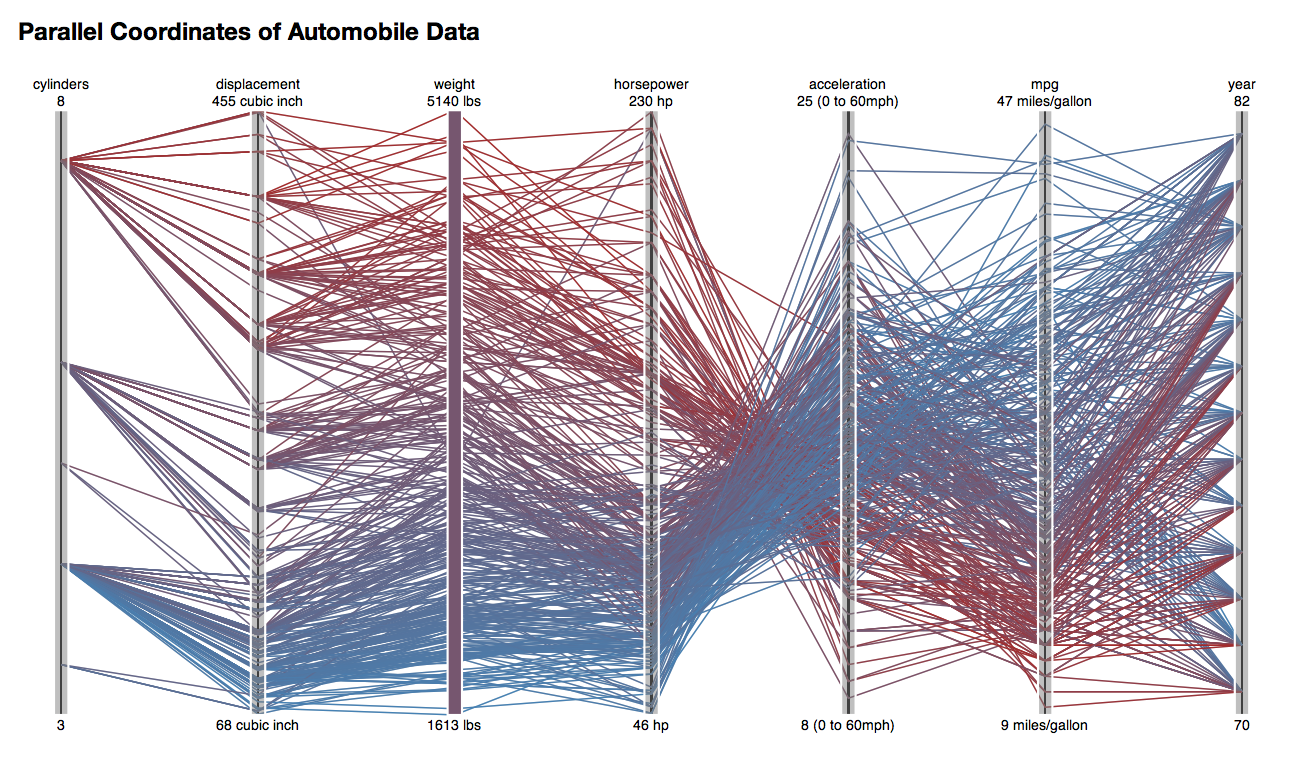
\includegraphics[width=1\textwidth]{parallel_coordinates}
\caption{Parallel Coordinates of Automobile Data}
\label{fig:parallel-coordinates}
\end{figure}

\subsection{Tree}
%%%-----------------------------------------------------------------------------

Tree structures or hierarchies describe parent-child relationships and are composed out of nodes that are connected through links. The topmost node in a tree (which will not have a parent) is called the root node, whereas lower level ones (which have no children) are called leaf nodes. Example tree datasets include spatial entities such as countries, software package hierarchies and genealogies.

\begin{figure}
\centering
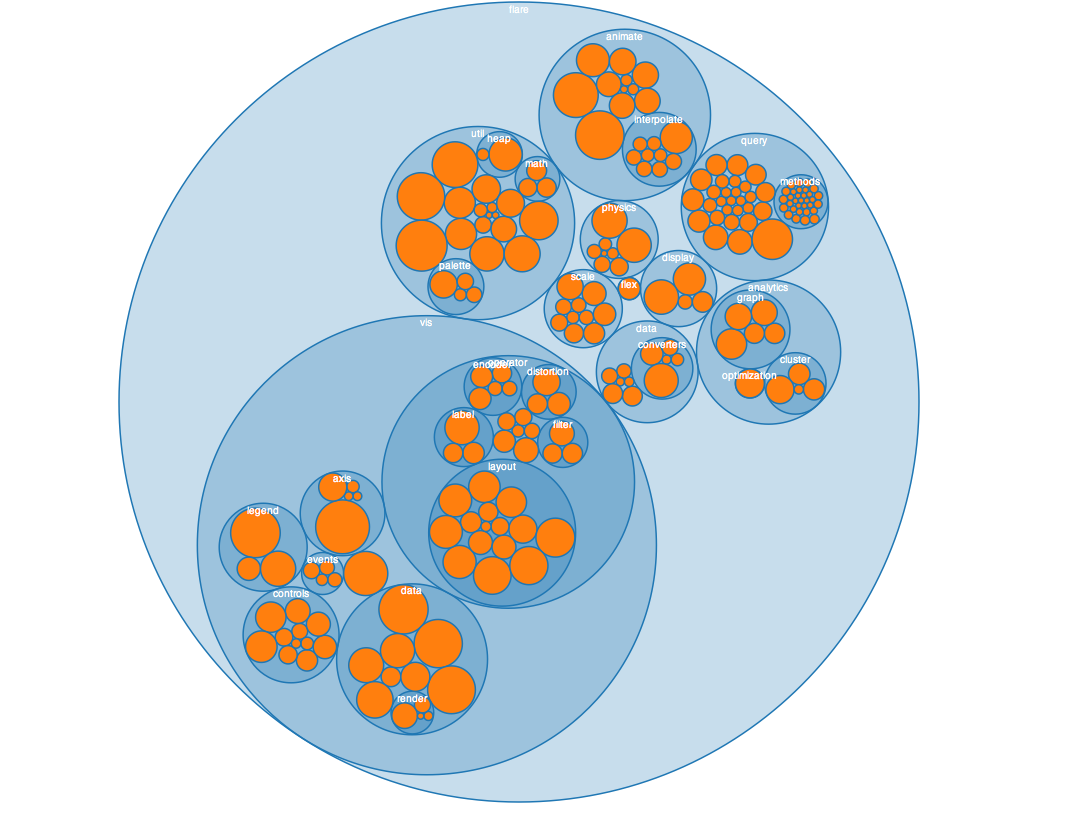
\includegraphics[width=1\textwidth]{nested_circles}
\caption{Nested Circles Layout of the Flare Package Hierarchy}
\label{fig:nested_circles}
\end{figure}


\SuperPar User Problems:

\begin{itemize}
\item How many levels does the tree have?
\item How many children does an item have?
\end{itemize}


\SuperPar Examples:

\begin{itemize}
\item \textbf{Sunbursts} (Figure~\ref{fig:sunburst}) are radial space-filling layouts for tree structures~\cite{VisualizationZoo:2010}.
\item \textbf{Nested Circles} (Figure~\ref{fig:nested_circles}) can also be used to visualize tree hierarchies by employing a \emph{circle-packing algorithm}~\cite{VisualizationZoo:2010}.
\end{itemize}

\begin{figure}
\centering
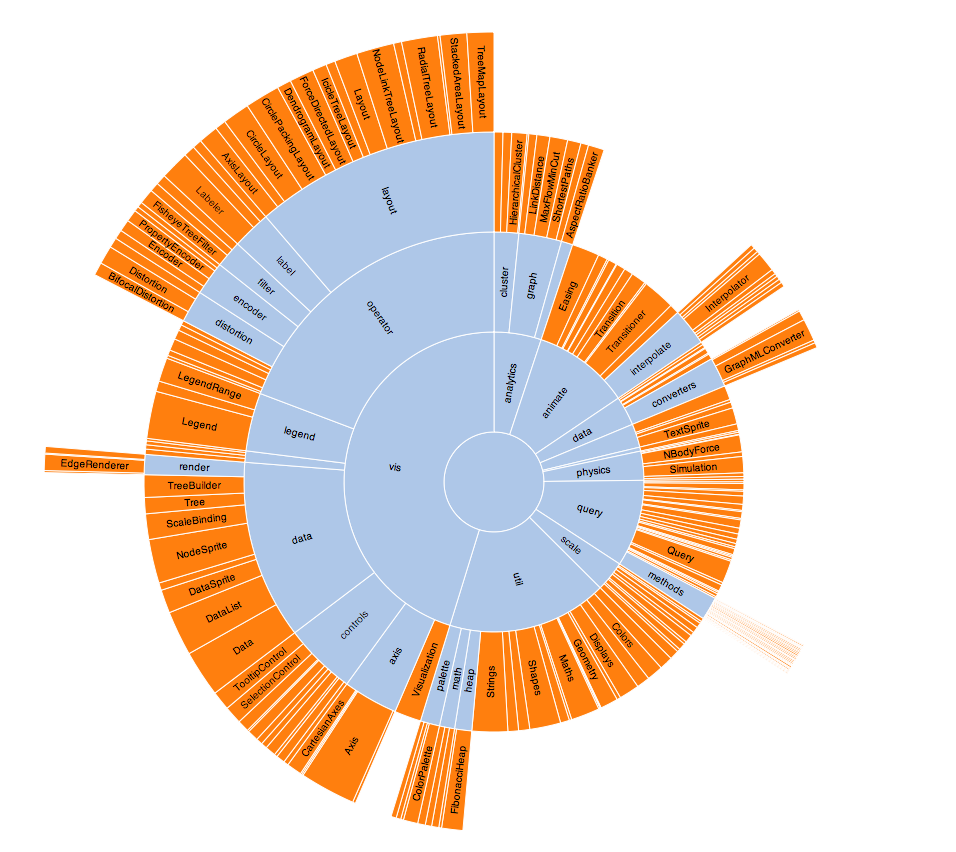
\includegraphics[width=1\textwidth]{sunburst}
\caption{Sunburst Layout of the Flare Package Hierarchy}
\label{fig:sunburst}
\end{figure}


\subsection{Network}
%%%-----------------------------------------------------------------------------

\begin{figure}
\centering
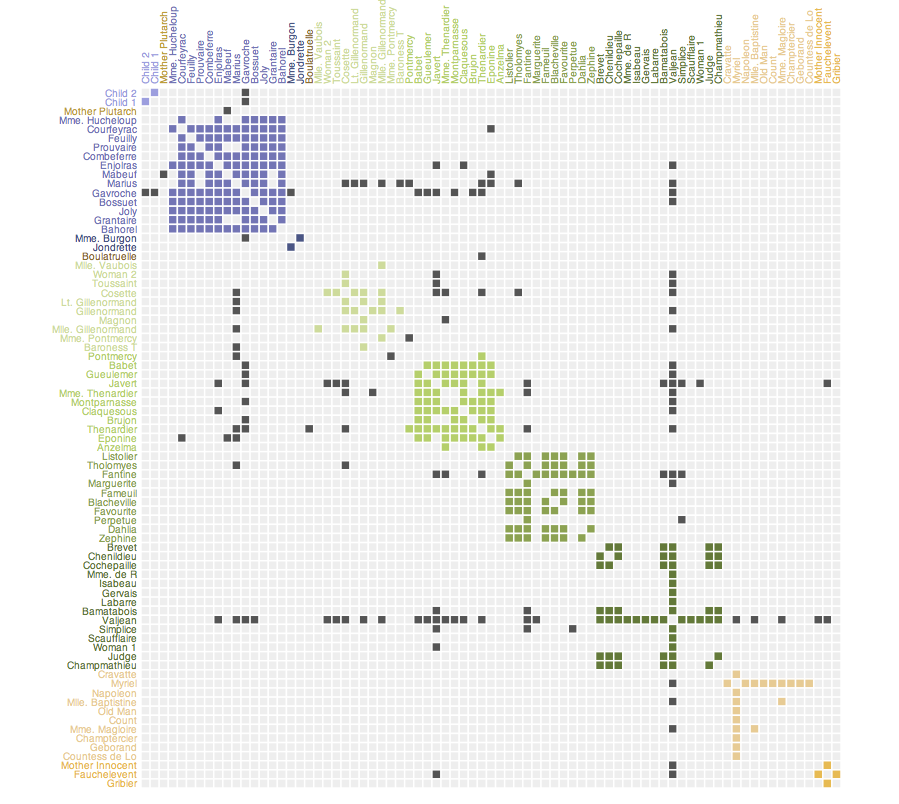
\includegraphics[width=1\textwidth]{matrix-view}
\caption{Matrix View of Les Miserables Character Co-occurrences}
\label{fig:matrix-view}
\end{figure}

One aspect of data that users wish to explore through visualization is \emph{relationship}. Networks are a data structure that capture such relationships using nodes that are connected through edges. Networks are also referred to as graphs in mathematical terminology. Social Networks (who is friend of whom) or workflow descriptions are examples for network datasets. Networks are hard to visualize because of their arbitrary complex structure. The central challenge is the computation of an effective layout, including tasks such as reducing the number of edge-crossings in order to be easily readable by the viewer.

\SuperPar User Problems:

\begin{itemize}
\item Which items are related to a particular item of interest?
\item Which is the shortest or least costly path connecting two items?
\end{itemize}


\SuperPar Examples:

\begin{itemize}
\item \textbf{Force directed layouts} (Figure~\ref{fig:force-directed-layout}) are a common approach to network visualization by modeling the graph as a physical system. This is achieved by assigning forces among the set of edges and the set of nodes~\cite{VisualizationZoo:2010}.
\item \textbf{Matrix Views} (Figure~\ref{fig:matrix-view}) represent linked data according to a graph's adjacency matrix.
\end{itemize}

\begin{figure}
\centering
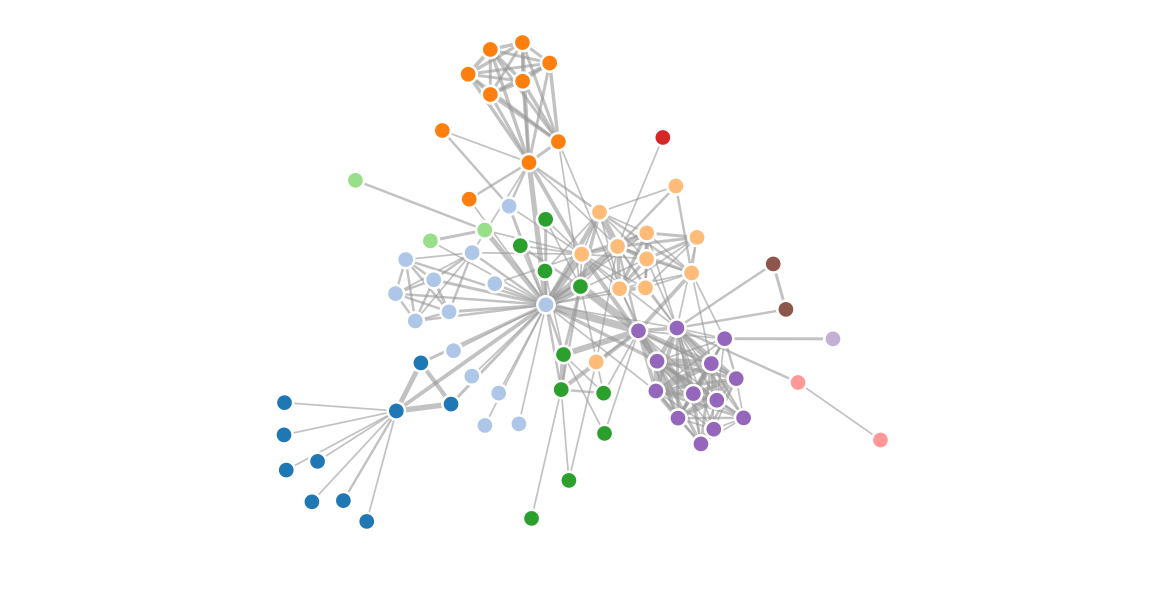
\includegraphics[width=1\textwidth]{force-directed-layout}
\caption{Force Directed Layout of Les Miserables Character Co-occurrences}
\label{fig:force-directed-layout}
\end{figure}


\section{Summary}
%%%-----------------------------------------------------------------------------

The basic concepts of Information Visualization were introduced in this chapter. After taking a look at the \emph{Visualization Process} in general, illustrative examples were used to describe the \emph{Tasks} and \emph{Data Types} of Information Visualization according to Shneiderman~\cite{shneiderman96eyes}. Based on that fundamental knowledge, the next chapter is dedicated to the application of Information Visualization within web-based environments.

\end{english}